\documentclass[11pt]{amsart}
\usepackage[margin=1in]{geometry}
\usepackage{amsmath,amssymb,amsthm,booktabs,microtype}
\usepackage{tikz}
\usepackage[most]{tcolorbox}
\usepackage[colorlinks=true,linkcolor=blue,urlcolor=blue,citecolor=blue,
hypertexnames=false]{hyperref}

\newtheorem{theorem}{Theorem}
\newtheorem{corollary}{Corollary}
\newtheorem{lemma}[theorem]{Lemma}
\newtheorem{remark}[theorem]{Remark}
\newcommand{\Sph}{\mathbb S^2}
\newcommand{\cP}{\mathcal P}


\begin{document}


\title{A set of points with optimal $L^2$ spherical cap discrepancy}


\author{Carlos Beltr\'an, Jordi Marzo and Joaquim Ortega-Cerd\`a}


%\author{Carlos Beltr\'an}
\address{ Departamento de Matem\'aticas, Estad\'{\i}stica y Computaci\'on,
Universidad de Can\-ta\-bria, Avd. Los Castros s/n, 39005, Santander, Spain}
\email{beltranc@unican.es}


%\author{Jordi Marzo}
\address{Departament de Matem\`atiques i Inform\`atica, Universitat de
Barcelona \& Barcelona Graduate School of Mathematics, Gran Via 585, 08007,
Barcelona, Spain}
\email{jmarzo@ub.edu}

%\author{Joaquim Ortega-Cerd\`a}
\address{Departament de Matem\`atiques i Inform\`atica, Universitat de
Barcelona \& Barcelona Graduate School of Mathematics, Gran Via 585, 08007,
Barcelona, Spain}
\email{jortega@ub.edu}




\keywords{Discrepancy, Riesz energy, Optimal configurations, Spherical
harmonics, Sobolev worst case error}
\thanks{The last two authors are supported by grant PID2024-160033NB-I00 funded by MICIU/AEI/10.13039/501100011033 and by FEDER, UE. JOC is also supported by the 2024 ICREA 00142 grant by the Generalitat de Catalunya.}


\begin{abstract}

We introduce an explicit deterministic collection of $N$ spherical points, $\cP_N\subset\mathbb S^2$, that we call the {\em deterministic Diamond points}. For every $0<\alpha<2$ we prove that there exists a constant $C_\alpha>0$ such that
\[ 0\leq \frac{2^{\alpha+1}}{\alpha+2}N^2-\sum_{x,y\in\cP_N}|x-y|^\alpha \le C_\alpha N^{1-\alpha/2}. \]
This result shows that $\cP_N\subset\mathbb S^2$ has a Riesz energy deficit of optimal order in this range of the parameter. In particular, for $\alpha=1$, Stolarsky's invariance principle implies that $\cP_N\subset\mathbb S^2$ has $L^2$ spherical cap discrepancy of asymptotically optimal order
\[ D_{L^2}^C(\mathcal P_N)\asymp N^{-3/4}, \]
making it, to our knowledge, the first explicit configuration proved to have this property. More generally, our result implies that the point set $\cP_N$  has Sobolev $H^{s}(\Sph)$ worst-case error of optimal order for all $1<s<2$.
\end{abstract}
\maketitle

\section{Introduction and results}

Many different quantities have been used to measure the regularity of discrete point sets. One of the most popular is the so-called $L^2$ spherical cap discrepancy, defined for a finite set $X\subset \Sph$ by
\[ D_{L^2}^C(X)=\sqrt{\int_{-1}^{1}\int_{\Sph}\left| \frac{\#(X\cap C(x,t))}{\#X}-\sigma(C(x,t)) \right|^2\, d\sigma(x)\,dt}, \]
where $C(x,t)=\{ y\in \Sph:\ x\cdot y\ge t \}$ is the spherical cap with center $x\in \Sph$ and geodesic radius $\arccos t$, and $\sigma$ denotes the normalized surface area measure on $\Sph$; see \cite{Beck, DT97, BHS19} and the references therein.

Of  particular interest is the asymptotic behavior of the discrepancy when the number of points tends to infinity. It was proved by Stolarsky \cite{Stolarsky}, using previous work by Ralph Alexander \cite{Alexander1972} , that there exists (non-explicit)
$N$-points sequences $X_N\subset \Sph$ such that
\begin{equation}\label{upper_bound}
D_{L^2}^C(X_N)\le C N^{-3/4}.
\end{equation}

The main ingredient in Stolarsky's proof is the subsequently called Stolarsky's invariance principle which gives a direct connection between the $L^{2}$ spherical cap discrepancy and the mutual sum of distances for points $x_1,\dots, x_N\in \Sph$ \cite{Stolarsky}:
$$4 D_{L^2}^C (\{ x_1,\dots, x_N \})^2=\int_{\Sph}\int_{\Sph}|x-y|d\sigma(x)d\sigma(y)-
\frac{1}{N^2}\sum_{i=1}^N \sum_{j=1}^N |x_i-x_j|,$$
see \cite{BDM18} for a recent elementary proof.

Improving earlier work by Stolarsky \cite{Stolarsky} and Harman \cite{Har82},
the upper bound (\ref{upper_bound}) was actually proved to be sharp by Beck in \cite{Beck} by showing that
there exists a
constant $c>0$ such that for all configurations of points
$$c N^{-3/4}\le D_{L^2}^C(X_N).$$
For a recent and elementary proof of this result, see \cite{BB25}.


Several authors have searched for configurations of points with asymptotic discrepancy of optimal order $N^{-3/4}$. For example, the expected discrepancy of jittered sampling and other random processes was proved to be of that order, see \cite{Beck,AZ15,BGM24}. %see \cite[Theorem 24 A],{Beck} as well as \cite{AZ15,BGM24}.
It was also proved in \cite{BSSW14,Skr19} that well separated spherical designs of optimal order, whose existence was established in a nonconstructive way in \cite{BRV13,BRV15}, also have this desired property.

However, to date, for all explicit, nonrandom configurations, the known discrepancy bounds are still quite far from optimal, being at best of order $N^{-1/2}$, which is the same order expected for uniform iid chosen points,
see \cite{ABD12,Eta21,FHM23} for theoretical bounds and \cite{HMS} for numerical experiments.


In this paper, we introduce a simple construction that derandomizes the Diamond ensemble introduced in \cite{Diamond} and whose $L^\infty$ discrepancy was studied in \cite{Eta21}. We refer to the resulting configurations as {\em deterministic Diamond points} and prove that their $L^2$ spherical cap discrepancy has optimal asymptotic growth. Our approach is similar to the construction that we introduced together with Uju\'e Etayo in \cite{BEMOC21} and to those of \cite{BL22,LG26}.
In \cite{BEMOC21}
it was proved that a deterministic and explicit family of points provides an example of the previously elusive set of zeros
of well-conditioned polynomials defined
by Shub and Smale, whose existence
had earlier been established by probabilistic methods \cite{SS93}. The underlying idea of this paper is similar.

A detailed construction of the deterministic Diamond points and some of their properties will be given in the next section. Briefly, we choose
a particular collection of parallels, symmetric with respect to the equator, and associate with each
parallel a band centered on it. The number of points assigned to each band
is chosen to be proportional to the area of the band and the points are placed equally spaced in the central parallel of each band.

To estimate the discrepancy of the deterministic Diamond points, we compare the discrete, semi-discrete (in parallels), and continuous contributions to
the energy
associated with the distance kernel. Our technique is valid for the more general problem of estimating the sum of the mutual distances to some power $0<\alpha<2$, which we will see also yields a corollary for Sobolev worst-case errors.


% Since the distance raised to a power is a conditionally negative definite kernel for exponents
% $0<\alpha<2$, we address the technically
% very close problem of determining whether the deterministic Diamond points have optimal distance-power energy for this range of $\alpha$. This approach further provides
% an interesting corollary
% concerning the worst-case error in Sobolev spaces.


\begin{theorem}\label{thm:main}
Let $\cP_N\subset\mathbb S^2$ be the $N$-set of deterministic Diamond points.  For every $0<\alpha<2$ there exists a constant $C_\alpha>0$ such that
\begin{equation}\label{theo:ineq}
0\leq  I_\alpha N^2-\sum_{x,y\in\cP_N}|x-y|^\alpha
   \le C_\alpha N^{1-\alpha/2},
\end{equation}
where $I_\alpha=\iint_{\Sph\times\Sph}|x-y|^\alpha
 \,d\sigma(x)d\sigma(y)=\frac{2^{\alpha+1}}{\alpha+2}.$
\end{theorem}

%The problem addressed in the previous theorem is therefore to estimate the second-order term in the asymptotic expansion of the Riesz energy of parameter $\alpha$ for $\cP_N$.
The bound in \eqref{theo:ineq} is of optimal order since the classical estimates of Wagner \cite{Wag90,Wag92} give
\begin{equation}\label{eq:optimalorder}
I_\alpha N^2-\max_{\#X=N} \sum_{x,y\in X}|x-y|^\alpha \asymp N^{1-\alpha/2}.
%\tag{1.2}
\end{equation}
For a simpler proof of the lower bound in the left-hand side of (\ref{eq:optimalorder}), and for a study of the conjectured constant accompanying the term $N^{1-\alpha/2}$ in \eqref{eq:optimalorder}, see \cite{BHS12,BHS19}. We also mention the recent work \cite{Steinerberger2026} for an upper bound attaining the conjectured quadratic coefficient for the exponent $\alpha=-2$, which is not in our range, but whose methods might also lead to sequences with proven low discrepancy points.




Taking $\alpha=1$ in equation \eqref{theo:ineq}, from Stolarsky's invariance principle we immediately get that the deterministic Diamond points have spherical $L^2$ discrepancy of optimal order:


\begin{corollary}\label{cor:main}
Let $\cP_N\subset\mathbb S^2$ be the $N$-set of deterministic Diamond points. There exist constants
$C,c>0$ such that
$$c N^{-3/4}\le D_{L^2}^C(\mathcal P_N)\le C N^{-3/4}.$$
\end{corollary}



Specializing \cite{BSSW14} to $\mathbb S^2$, we now introduce the notion of worst-case error for Sobolev spaces and the relation with our previous results. Given an integer $\ell\ge 0$, let $\mathcal{H}_\ell$ be the $(2\ell+1)$--dimensional vector space of eigenfunctions of the Laplace-Beltrami operator in $\mathbb S^2$, $\Delta,$ with eigenvalue $\lambda_\ell=\ell (\ell+1)$,
\begin{equation*}
-\Delta Y=\lambda_\ell Y,\;\;\;\; Y\in \mathcal{H}_{\ell}.
\end{equation*}
The space $\bigoplus_{\ell=0}^L \mathcal{H}_\ell$ of spherical harmonics of degree at most
$L$ on $\mathbb{S}^2$ has dimension $(L+1)^2$ and coincides with the space of degree at most $L$ polynomials on $\mathbb R^3$ restricted to $\mathbb S^2$.


Let $L^2(\mathbb{S}^2)$ be the Hilbert space of square integrable real functions in $\mathbb{S}^2$
with the inner product
\[
\langle f,g \rangle=\int_{\mathbb{S}^2} f(x)g(x)\,d\sigma(x),\;\;\; f,g\in L^2(\mathbb{S}^2).
\]
Then $L^2(\mathbb{S}^2)=\bigoplus_{\ell\ge 0} \mathcal{H}_\ell$ and the Fourier series expansion of a function $f \in L^2(\mathbb{S}^2)$ is given by
\begin{equation*}
f=\sum_{\ell,k} f_{\ell,k} Y_{\ell,k},\qquad f_{\ell,k}=\langle f,Y_{\ell,k} \rangle=\int_{\mathbb{S}^2} f\, Y_{\ell,k} \,d\sigma,
\end{equation*}
where $\{ Y_{\ell,k} \}_{k=-\ell}^{\ell}$ is an orthonormal basis of $\mathcal{H}_\ell.$

For $s\ge 0,$ the $L^2(\mathbb{S}^2)$-based Sobolev spaces of order $s$ are the Hilbert spaces
$$\mathbb{H}^{s}(\mathbb{S}^2)=\left\{ f\in L^2(\mathbb{S}^2)\;\;:\;\;
\sum_{\ell=0}^{+\infty}\sum_{k=-\ell}^{\ell} (1+\lambda_\ell)^s |f_{\ell,k}|^2<+\infty \right\},$$
with the norm
\begin{equation}\label{eq:sobolev}\| f \|_{\mathbb{H}^{s}(\mathbb{S}^2)}=\left( \sum_{\ell=0}^{+\infty}\sum_{k=-\ell}^{\ell} (1+\lambda_\ell)^s |f_{\ell,k}|^2  \right)^{1/2}.\end{equation}
The space
$\mathbb{H}^{s}(\mathbb{S}^2)$ is continuously embedded in the space of continuous functions $\mathcal{C}(\mathbb{S}^2)$ if $s >1.$ Our last result shows that deterministic Diamond points have optimal worst-case error for Sobolev spaces $H^s(\Sph)$ if $1<s<2.$ As in the case of the $L^2$ cap discrepancy, this is, to our knowledge, the first explicit configuration to
achieve this property.

\begin{corollary}\label{cor:wce}
Let $\cP_N\subset\mathbb S^2$ be the $N$-set of deterministic Diamond points. For $1<s<2$ there exists a constant
$C_s>0$ such that
$$\sup_{\| f \|_{\mathbb{H}^{s}(\mathbb{S}^2)}\le 1}
\left| \frac{1}{N}\sum_{x\in \cP_N}f(x)-\int_{\mathbb{S}^2}f(x)d\sigma(x) \right| \le C_s N^{-s/2}.$$
\end{corollary}

The asymptotic behavior in the corollary above is optimal because %for all families of N-points configurations
there is a lower bound for the worst-case error of the same order, see  \cite{BSSW14}. Corollary \ref{cor:wce} follows immediately from Theorem \ref{thm:main} and the following relation proved in \cite[(29)]{BSSW14} for $1<s<2$ (note that \cite{BSSW14} uses several norms in $\mathbb{H}^{s}(\mathbb{S}^2)$, but they are all equivalent to that of \eqref{eq:sobolev}): for some constant $C_s>0$,
$$\sup_{\| f \|_{\mathbb{H}^{s}(\mathbb{S}^2)}\le 1}
\left| \frac{1}{N}\sum_{x\in X_N}f(x)-\int_{\mathbb{S}^2}f(x)d\sigma(x) \right|^2\leq C_s\left(
I_{2s-2}-\frac{1}{N^2}\sum_{i=1}^N\sum_{j=1}^N|x_i-x_j|^{2s-2}\right).$$



%==============================================================
%==============================================================

%==============================================================
%==============================================================

%==============================================================
%==============================================================

%==============================================================
%==============================================================

% For $0<\alpha<2$ define the maximal distance-power energy
% \[
%  \mathcal M_\alpha(N)=\max_{\#X=N}
%  \sum_{\substack{x,y\in X\\x\ne y}}|x-y|^\alpha.
% \]
% The continuous energy of normalized surface area $\sigma$ is
% \begin{equation}\label{eq:continuous}
%  I_\alpha:=\iint_{\Sph\times\Sph}|x-y|^\alpha
%  \,d\sigma(x)d\sigma(y)=\frac{2^{\alpha+1}}{\alpha+2}. %\tag{1.1}
% \end{equation}
% Indeed, for fixed $x\in\Sph$ the variable $u=x\cdot y$ is uniform on
% $[-1,1]$ under $d\sigma(y)$, and hence
% \[
%  I_\alpha=\frac12\int_{-1}^1(2-2u)^{\alpha/2}\,du
%  =\frac14\int_0^4v^{\alpha/2}\,dv
%  =\frac{2^{\alpha+1}}{\alpha+2}.
% \]
% Since $|x-y|^\alpha$ is a conditionally negative definite kernel,
% $\sum_{x\ne y}|x-y|^\alpha\le I_\alpha N^2$.  The classical estimates of
% Wagner, summarized in \cite[Theorem~3.6]{HMS}, give
% \begin{equation}\label{eq:optimalorder}
%  I_\alpha N^2-\mathcal M_\alpha(N)\asymp_\alpha
%  N^{1-\alpha/2}.                                     %\tag{1.2}
% \end{equation}
% The conjecture of Brauchart--Hardin--Saff predicts a limiting coefficient
% expressed through the triangular-lattice Epstein zeta function
% \cite{BHS}.  That coefficient is not known in general.

% The case $\alpha=1$ has an additional discrepancy interpretation.
% Stolarsky's invariance principle \cite{Stolarsky} identifies
% \[
%  \frac43N^2-\sum_{x\ne y}|x-y|
% \]
% with four times $N^2$ times the squared spherical-cap $L^2$ discrepancy.
% Together with Beck's sharp discrepancy estimates \cite{Beck}, this gives the classical
% extremal result
% \[
%  \max_{\#X=N}\sum_{x\ne y\in X}|x-y|
%  =\frac43N^2-\Theta(\sqrt N).
% \]
% The expected refinement of Brauchart--Hardin--Saff is
% \[
%  \max_{\#X=N}\sum_{x\ne y\in X}|x-y|
%  =\frac43N^2-c_*\sqrt N+o(\sqrt N),
%  \qquad
%  c_*=-\left(\frac{8\pi}{\sqrt3}\right)^{1/2}
%  \zeta_\Lambda(-1)=0.79851125\ldots,
% \]
% where $\Lambda$ is the unit-edge triangular lattice.  Neither existence of
% this limit nor the predicted value is known.  Our theorem proves the optimal
% order for the explicit BEMOC set; it does not identify its full limiting
% coefficient.

\section{Notation and construction of the deterministic Diamond points}
We will use the asymptotic notation: for two collections of numbers $A(\eta,\nu,\ldots)$ and $B(\eta,\nu,\ldots)$, where $\eta,\nu,\ldots$ are any parameters, the expression
\[
A(\eta,\nu,\ldots)\asymp B(\eta,\nu,\ldots)
\]
means that there exist universal constants $0<c<C$ such that
\[
c A(\eta,\nu,\ldots)\leq B(\eta,\nu,\ldots)\leq CA(\eta,\nu,\ldots),\quad \text{for all choices of the parameters.}
\]
If we only have  the upper bound $B(\eta,\nu,\ldots)\leq CA(\eta,\nu,\ldots)$ then we write
\[
B(\eta,\nu,\ldots)\lesssim A(\eta,\nu,\ldots)
\]
The symbols $\asymp_\eta$ and $\lesssim_\eta$ are used if the constants depend on the parameter $\eta$.


The  unspecified constants in Theorem \ref{thm:main} allow us to assume in the proof that $N\geq N_0$ for any fixed positive integer $N_0$. We now give the construction of our point set for every $N\geq4$, although the proof will assume $N\geq 1024$, that implies $M\geq16$ in \eqref{eq:rj} below.
The construction is similar to that of \cite[Section 4.1]{Diamond} or \cite[Section 3]{LG26} but excludes the poles and avoids the choice of random phases. Fix
$N\ge4$ and put
\begin{equation}\label{eq:rj}
 M=\left\lfloor\sqrt{N/4}\right\rfloor,\qquad
 r_j=4j\quad(1\le j<M),\qquad
 r_M=N-2\sum_{j=1}^{M-1}r_j .
\end{equation}
%More generally, our proof below is valid with the less restrictive hypotheses
%\[
%cj\leq r_j\leq Cj, 1\leq j\leq M, \text{ for some constants }C>c>0,
%\]
%but we stick to the use of \eqref{eq:rj} to avoid the introduction of extra notation.

Note that
\[
4M^2\leq N\leq 4(M+1)^2-1=4M^2+8M+3,\text{ and then }N\asymp M^{2}.
\]
Extend symmetrically by $r_{M+j}=r_{M-j}$ for $1\le j<M$.

We denote the parallels in $\Sph$ by
$$Q_{h}=\{(x,y,z)\in \Sph : z=h \},\;\;\;-1\leq h \leq 1.$$
Let
\[
H_j=1-\frac{2}{N}\sum_{k=1}^j r_k\quad 0\leq j\leq 2M-1,
\]
which define the bands
$$\mathcal B_j=\{ (x,y,z)\in \Sph \;\:\; H_j\le z\le H_{j-1} \},$$
where $\mathcal B_1,\mathcal B_{2M-1}$ are spherical caps. Then $\Sph=\bigcup_{j=1}^{2M-1} \mathcal B_j$ and
\[
\sigma(\mathcal B_j)=\frac{H_{j-1}-H_j}{2}=\frac{r_j}{N},\quad 1\leq j\leq 2M-1.% \text{ and  }
%\;H_{M+j-1}=-H_{M-j}.
\]
The parallels bounding each band $\mathcal B_j$ are precisely $Q_{H_{j-1}}$ and $Q_{H_{j}}$. We consider also the central parallels $Q_{h_j}$ with heights
\[
h_j=\frac{H_{j-1}+H_j}{2}=H_{j-1}-\frac{r_j}{N}=H_{j}+\frac{r_j}{N}=1-\frac{2}{N}\sum_{k=1}^{j-1}
r_k
-\frac{r_j}{N},
\]
for $1\leq j\leq 2M-1,$ and observe that $h_M=0$ and $h_{M+j}=-h_{M-j}$ for $j=1,\dots, M-1.$

 In order to construct $\cP_N$, place $r_j$ equally spaced points in each parallel of height $h_j$. Hence, these points are the $r_j$ vertices of a regular polygon, equivalently, up to rotation and scaling, they form a set of roots of unity in the circumference defined by the
parallel. The points can be rotated in any desired way, or forced to have one of them in any predefined meridian. In order to fix some criteria, we determine the set completely by forcing that in each parallel there exists one point such that its first coordinate is positive and its second coordinate vanishes, but we point that this choice is not important for the proof below, and hence our main result and corollaries also hold for any arbitrary rotation of the points in each parallel.

For later use, observe that
\begin{align*}
h_j=&1-\frac{4j^2}N,\quad 1\leq j\leq M-1,\\
 \sum_{j=1}^{M-1}r_j
 =&4\frac{(M-1)M}{2}=2M(M-1),\\
 r_M&=N-4M(M-1),
\end{align*}
and hence $4M\le r_M\le12M+3.$ Thus the number of points in the equator is of order $M$, and the total number of points is $N$. There are a total of $2M-1$ occupied parallels. See Figure \ref{fig:bemoc} for a graphical representation of the  points.

Each parallel $Q_j=Q_{h_j}$ is a circumference of radius $\rho_j=\sqrt{1-h_j^2}$. Note that
% \[
% \rho_j\asymp\begin{cases}\frac{2j}{\sqrt N}& 1\leq j\leq M-1\\
% 1&j=M\\
% \frac{2(M-j)}{\sqrt N}&M+1\leq j\leq 2M-1
% \end{cases}
% \]

%=================================================

\begin{figure}[t]
\centering
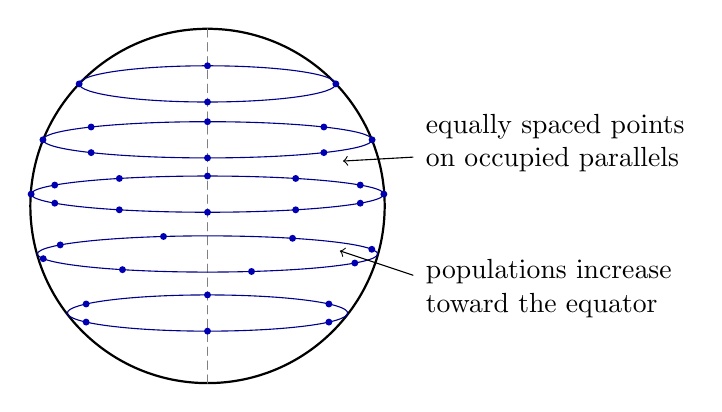
\begin{tikzpicture}[scale=1.0,line cap=round,line join=round]
  \def\R{2.25}
  \draw[thick] (0,0) circle (\R);
  \draw[densely dashed,gray] (0,-\R) -- (0,\R);
  \foreach \y/\rx/\step/\shift in
   {1.55/1.63/90/0,.84/2.09/45/0,.15/2.24/30/0,
    -.61/2.16/45/15,-1.36/1.78/60/30}{
    \draw[blue!55!black] (0,\y) ellipse [x radius=\rx,y radius=.23];
    \foreach \a in {0,\step,...,359}
      \fill[blue!70!black]
       ({\rx*cos(\a+\shift)},{\y+.23*sin(\a+\shift)}) circle (1.25pt);
  }
  \node[align=left,anchor=west] at (2.65,.80)
    {equally spaced points\\on occupied parallels};
  \draw[->] (2.61,.62)--(1.72,.57);
  \node[align=left,anchor=west] at (2.65,-1.05)
    {populations increase\\toward the equator};
  \draw[->] (2.61,-.88)--(1.68,-.57);
\end{tikzpicture}
\caption{Schematic deterministic Diamond configuration.  There are $O(\sqrt N)$ occupied
parallels, and the phases of each polygon can be chosen arbitrarily or fixed to any desired standard.}
\label{fig:bemoc}
\end{figure}

%=================================================
%In particular, we have
\begin{equation}\label{eq:geometry}
 r_j\asymp M\rho_j,\;1\leq j\leq 2M-1,\quad  \text{ and  } \quad \sum_{j=1}^{2M-1}\rho_j\asymp M.                    %\tag{1.3}
\end{equation}



\section{Proof of Theorem \ref{thm:main}}

%The strategy is similar to the one in \cite{BEMOC21}.
%To prove our result
%we will add and subtract the energy
%given by the semi-discrete energy defined
%on the union
%of the $2M-1$ occupied parallels as a sum of the (conveniently normalized)
%uniform probability measures on each of them.

We will use the following  well known integral formula, valid for any integrable function $f:\mathbb S^2\to\mathbb R$:
\begin{equation}\label{eq:integralaintervalo}\int_{\mathbb S^2}f(x)d\sigma(x)=\frac{1}{2}\int_{-1}^1 \frac{1}{2\pi}\int_0^{2\pi} f(\sqrt{1-t^2}\cos \theta,\sqrt{1-t^2}\sin \theta,t)d\theta dt.
\end{equation}
We need to bound the LHS in \eqref{theo:ineq}, which is the error between the Riesz energy of the measure $N\sigma$ and the Riesz energy of the fully discrete measure $\sum_{x\in\mathcal P_N}\delta_x.$

For the parallel with height $z$ we denote as $U_z$ the uniform probability measure on the circle at height $z$ and define $\nu=\sum_jr_jU_{h_j}.$ Then its energy is
\begin{equation}\label{eq:energianu}E_\alpha[\nu]=\int_{\Sph}\int_{\Sph}|x-y|^\alpha d\nu(x)d\nu(y)=\sum_{j,k}r_jr_k
F_\alpha(h_j,h_k)\end{equation}
where
\begin{equation}\label{eq:Falpha}
 F_\alpha(s,t)=\int_{\Sph}\int_{\Sph}|x-y|^\alpha d U_{s}(x)d U_{t}(y)=\frac1{2\pi}\int_0^{2\pi}
 \left(2-2st-2\sqrt{1-s^2}\sqrt{1-t^2}\cos\theta
 \right)^{\alpha/2}d\theta.
\end{equation}


Given any two (possibly equal) parallels $Q_j$ and $Q_k$ in our construction, write
$$\Sigma_{\alpha,jk}=
\sum_{x \in \mathcal P_N\cap Q_{j}}\sum_{y \in \mathcal P_N\cap Q_{k}}|x-y|^\alpha,\;\;\mbox{so that}\;\;
 \sum_{x,y\in \mathcal{P}_N}|x-y|^\alpha
 =\sum_{j,k}\Sigma_{\alpha,jk}.$$
We then have the decomposition
\begin{equation}\label{eq:decomp}
\text{LHS in \eqref{theo:ineq}}=I_\alpha N^2-\sum_{x,y\in \mathcal{P}_N}|x-y|^\alpha
 =A_{\alpha,N}+B_{\alpha,N},             %\tag{2.1}
\end{equation}
where
\begin{align*}
 A_{\alpha,N}&=I_\alpha N^2-E_\alpha[\nu],\\
 B_{\alpha,N}&=\sum_{j,k}\left(r_jr_kF_\alpha(h_j,h_k)
                    -\Sigma_{\alpha,jk}\right).
\end{align*}

\noindent Observe that $|x-y|^\alpha$ is strictly
conditionally negative definite for $0<\alpha<2$ (see for example \cite[Th. 4.4.7]{BHS19}).  Thus, for every signed
measure $\eta$ of total mass zero,
\[
 \iint |x-y|^\alpha\,d\eta(x)d\eta(y)\le0.
\]
Applying this with $\eta=\nu-N\sigma$ gives $A_{\alpha,N}\ge0$; the identical computation
with the atomic point measure gives that the LHS in \eqref{theo:ineq} is also nonnegative.


In subsequent sections we prove that both $A_{\alpha,N}$ and $B_{\alpha,N}$ in
the decomposition
(\ref{eq:decomp}) are bounded above by a constant depending on $\alpha$ times $N^{1-\alpha/2}$, see lemmas \ref{lem:BalphaN} and \ref{lem:latitude}, which proves Theorem \ref{thm:main}.






\subsection{The bound of $B_{\alpha,N}$}


%============================================
In this section, we prove the following result.
\begin{lemma}\label{lem:BalphaN}
For $0<\alpha<2$,
\begin{equation*}%\label{eq:BalphaN}
    B_{\alpha,N}\lesssim_\alpha N^{1-\alpha/2}
\end{equation*}
\end{lemma}
We will use the following auxiliary result.
\begin{lemma}\label{lem:trap}
Let $0<\alpha<2$ and $G(\theta)=(A-B\cos\theta)^{\alpha/2}$ with $A\ge B\ge0$.  For all
integers $L\ge1$ and all phases $\phi$,
\[
 \left|\frac1L\sum_{k=0}^{L-1}G(\phi+2\pi k/L)
 -\frac1{2\pi}\int_0^{2\pi}G\right|
 \lesssim_\alpha B^{\alpha/2}L^{-1-\alpha}.             %\tag{4.1}
\]
\end{lemma}

%==============================================


\begin{proof}
See Appendix \ref{appendix1}.
\end{proof}

\begin{proof}[Proof of Lemma \ref{lem:BalphaN}]

We apply the triangle inequality and estimate each summand
\[ \left|r_jr_kF_\alpha(h_j,h_k) -\Sigma_{\alpha,jk}\right| \]
separately. Recall that at the parallel $Q_j$ there are $r_j$ points of $\mathcal P_N$ lying on a circle of radius $\rho_j$. The angular coordinates of these points can be written as \[ \theta_{j,\ell} = \theta_{j,0}+\frac{2\pi \ell}{r_j}, \qquad \ell=0,\dots,r_j-1, \] for some (unimportant) phase $\theta_{j,0}\in[0,2\pi)$. Define
\begin{equation*}%\label{function_G}
G(\theta) = (A-B\cos\theta)^{\alpha/2}, \qquad A=2-2h_jh_k, \qquad B=2\rho_j\rho_k.
\end{equation*}
Observe that $A\ge B\ge 0$ and there is  equality $A=B$ if and only if $j=k.$

Then the value of $|x-y|^\alpha$ for two points $x,y\in\mathcal P_N$ lying on two fixed parallels $Q_j$ and $Q_k$ is $G(\theta_{j,\ell}-\theta_{k,\ell'})$ for some $\ell\in\{0,\dots,r_j-1\}$ and $\ell'\in\{0,\dots,r_k-1\}$. Therefore,
\begin{equation*} \Sigma_{\alpha,jk} = \sum_{\ell=0}^{r_j-1}\sum_{\ell'=0}^{r_k-1} G(\theta_{j,\ell}-\theta_{k,\ell'})
= \sum_{\ell=0}^{r_j-1}\sum_{\ell'=0}^{r_k-1} G\left( \theta_{j,0}-\theta_{k,0} + 2\pi\left(\frac{\ell}{r_j}-\frac{\ell'}{r_k}\right) \right).
\end{equation*}
Let
\[ L=\mathrm{lcm}(r_j,r_k) \qquad\text{and}\qquad d=\mathrm{gcd}(r_j,r_k) \]
denote, respectively, the least common multiple and the greatest common divisor of $r_j$ and $r_k$. Among the $r_jr_k$ angles
$2\pi\left(\frac{\ell}{r_j}-\frac{\ell'}{r_k}\right)$
appearing in the sum above, only $L$ are distinct modulo $2\pi$, and each of them occurs exactly $d$ times. Hence,
\[
\Sigma_{\alpha,jk} = d\sum_{u=0}^{L-1} G\left(\phi+\frac{2\pi u}{L}\right), \qquad \phi=\theta_{j,0}-\theta_{k,0}. \]
Since $r_jr_k=dL$ and
\[ F_\alpha(h_j,h_k) = \frac{1}{2\pi}\int_0^{2\pi}G(\theta)\,d\theta, \]
subsequently using Lemma~\ref{lem:trap} and the relation $r_j\asymp M\rho_j$ from \eqref{eq:geometry}, we finally obtain

\begin{align*} %\label{eq:aux1}
|r_jr_kF_\alpha(h_j,h_k) -\Sigma_{\alpha,jk}|  =& dL\left| \frac{1}{2\pi}\int_0^{2\pi}G(\theta)\,d\theta - \frac{1}{L}\sum_{u=0}^{L-1} G\left(\phi+\frac{2\pi u}{L}\right) \right|\\\nonumber
    \lesssim_\alpha&
        (\rho_j\rho_k)^{\alpha/2}
    \frac{d^{1+\alpha}}{(r_jr_k)^\alpha}
    \lesssim_\alpha
     M^{-\alpha}
    \frac{d^{1+\alpha}}
         {(r_jr_k)^{\alpha/2}}\nonumber.
\end{align*}

Trivially observe that for any positive integer $n$, there exist at most $3$ occupied parallels that have exactly $n$ points (one in the northern hemisphere, another one in the southern hemisphere, and eventually the equator). Hence, since $r_M\leq 15M$,
\begin{align*}
    |B_{\alpha,N}|
    \lesssim_\alpha
    M^{-\alpha}
    \sum_{1\leq u,v\leq 15M}
    \frac{\mathrm{gcd}(u,v)^{1+\alpha}}
         {(uv)^{\alpha/2}}.
\end{align*}
It remains to estimate the last double sum. For every pair $u,v$, write
uniquely
\[
    u=da,\qquad v=db,\qquad \mathrm{gcd}(a,b)=1,
\]
where $d=\mathrm{gcd}(u,v)$. Then
\[
    \frac{\mathrm{gcd}(u,v)^{1+\alpha}}{(uv)^{\alpha/2}}
    =
    \frac{d}{(ab)^{\alpha/2}}.
\]
Therefore
\begin{align*}
    \sum_{1\leq u,v\leq 15M} &
    \frac{\mathrm{gcd}(u,v)^{1+\alpha}}{(uv)^{\alpha/2}}
    =
    \sum_{\substack{a,b\geq1\\\mathrm{gcd}(a,b)=1}}
    \frac{1}{(ab)^{\alpha/2}}
    \sum_{1\leq g\leq 15M/\max(a,b)}g
    \\
    \lesssim & M^2 \sum_{\substack{a,b\geq1\\\mathrm{gcd}(a,b)=1}}
    \frac{1}{(ab)^{\alpha/2}\max(a,b)^2}
    \lesssim M^2\sum_{a,b\geq1}
    \frac{1}{(ab)^{1+\alpha/2}}
    =M^2\zeta\left(\frac{\alpha}{2}+1\right)^2
    \lesssim_\alpha M^2.
\end{align*}

Restoring the factor $M^{-\alpha}$ gives
\[
    |B_{\alpha,N}|
    \lesssim_\alpha M^{2-\alpha}\asymp N^{1-\alpha/2},
\]
as claimed.

\end{proof}

%================================================

%==========================================


\subsection{Bound of $A_{\alpha,N}$}

We will compare the union of rings measure $\nu=\sum_j r_jU_{h_j}$ with $N\sigma$  after projecting both
measures onto the height variable. Since the normalized surface measure on
$\mathbb S^2$ has height density $dt/2$, define
\[
 \lambda=\frac N2\mathbf 1_{[-1,1]}(t)\,dt,
 \qquad
 \nu_z=\sum_j r_j\delta_{h_j}.
\]
Thus $\lambda$ is the height projection of $N\sigma$, whereas $\nu_z$ is the
height projection of $\nu$.

For $1\le j\le 2M-1$, let
\[
 B_j=[H_j,H_{j-1}],
\]
then, from \eqref{eq:integralaintervalo}, $\lambda(B_j)=N\sigma(\mathcal B_j)$.
Define the following measures on $B_j$
\begin{align*}
 \nu_j={}&r_j\delta_{h_j},\quad\Rightarrow \nu_z=\sum\nu_j,\\
 \lambda_j={}&\frac N2\mathbf 1_{B_j}(t)\,dt,\quad\Rightarrow \lambda=\sum\lambda_j,\\
 \mu_j={}&\lambda_j-\nu_j.
\end{align*}
% so we trivially have
% \[
%  \mu:=\nu_z-\lambda=\sum_{j=1}^{2M-1}\mu_j.
% \]
We next rewrite $A_{\alpha,N}$ as a sum over the bands. First, note from \eqref{eq:integralaintervalo} that
\begin{align*}
    I_\alpha=E_\alpha[\sigma]=&\int_{\Sph}\int_{\Sph}|x-y|^\alpha d \sigma(x)d \sigma(y)\\
    =&\frac1{N^2}\int_{-1}^1\int_{-1}^1F_\alpha(s,t)\,d\lambda(t)\,d\lambda(s)\\
=&\frac1{N^2}\sum_{j,k=1}^{2M-1}\int_{B_j}\int_{B_k}F_\alpha(s,t)\,d\lambda_k(t)\,d\lambda_j(s)
\end{align*}
% Both $\nu_z$ and $\lambda$ have mass $N$. Furthermore, from the first equality in \eqref{eq:Falpha},
% \begin{align*}
%  \int_{-1}^1F_\alpha(s,t)\,d\lambda(t)=&
%  \int_{-1}^1\int_{\Sph}\int_{\Sph}|x-y|^\alpha d U_{s}(x)d U_{t}(y)\,d\lambda(t)
%  \\
%  =&
% \int_{\Sph}\int_{\Sph}|x-y|^\alpha d U_{s}(x)(x)\int_{-1}^1d U_{t}(y)\,d\lambda(t)
% \\
%  =&
% N\int_{\Sph}\int_{\Sph}|x-y|^\alpha d\sigma(y)d U_{s}(x)
%  \\
%  =&NI_\alpha,
% \end{align*}
% is independent of $s$, the last equality by rotational invariance. Hence,
% \begin{align*}
% I_\alpha N^2=&\frac N2\int_{-1}^1\int_{-1}^1F_\alpha(s,t)\,d\lambda(t)\,ds\\=&\int_{-1}^1\int_{-1}^1F_\alpha(s,t)\,d\lambda(t)\,d\lambda(s)\\
% =&\sum_{j,k=1}^{2M-1}\int_{B_j}\int_{B_k}F_\alpha(s,t)\,d\lambda_k(t)\,d\lambda_j(s).
% \end{align*}
We also have from \eqref{eq:energianu}:
\begin{equation*}
 E_\alpha[\nu]=\sum_{j,k=1}^{2M-1}r_jr_k F_\alpha(h_j,h_k)
=\sum_{j,k=1}^{2M-1}\int_{B_j}\int_{B_k} F_\alpha(s,t)\,d\nu_k(t)\,d\nu_j(s).
\end{equation*}
Rotational invariance gives
\[
 \int_{-1}^1F_\alpha(s,t)\,d\lambda(t)=NI_\alpha
 \qquad(-1\le s\le1).
\]
Thus the mixed term in the energy expansion vanishes for
$\mu:=\lambda-\nu_z=\sum_j\mu_j$, which has total mass zero.
We thus have
\begin{equation}\label{eq:latitude-decomposition}
 A_{\alpha,N}
 =I_\alpha N^2-E_\alpha[\nu]
 =-\sum_{j,k=1}^{2M-1}
   \int_{B_j}\int_{B_k}F_\alpha(s,t)\,d\mu_k(s)d\mu_j(t).
                                                               %\tag{5.9}
\end{equation}



We will use the following technical lemma.

\begin{lemma}\label{lem:blocks}
Let $0<\alpha<2$. There exists a constant $C_\alpha$ with the following properties.

If the two bands have comparable scales,
\[
 \frac{r_j}{8}\le r_k\le 8 r_j,
\]
then
\begin{equation}\label{eq:comparableblock}
 \left|
 \int_{B_j}\int_{B_k}F_\alpha(s,t)\,d\mu_k(s)d\mu_j(t)
 \right|
 \le C_\alpha\frac{r_j}{M^\alpha}
 (1+|j-k|)^{\alpha-3}.                               %\tag{5.12}
\end{equation}

If $r_k> 8 r_j$ and the two bands are on the same side of the equator
(that is, either $j,k<M$ or $j,k>M$), then
\begin{equation}\label{eq:farblock}
 \left|
 \int_{B_j}\int_{B_k}F_\alpha(s,t)\,d\mu_k(s)d\mu_j(t)
 \right|
 \le C_\alpha\frac{r_j^3}{M^\alpha r_k^{5-\alpha}}.
                                                               %\tag{5.13}
\end{equation}

If $r_k>8r_j$ and the bands are not on the same side
of the equator, including the case in which one of the indices is $M$,
then
\begin{equation}\label{eq:oppositeblock}
 \left|
 \int_{B_j}\int_{B_k}F_\alpha(s,t)\,d\mu_k(s)d\mu_j(t)
 \right|
 \le C_\alpha\frac{r_j^3r_k^3}{M^8}.                %\tag{5.14}
\end{equation}
\end{lemma}
\begin{proof}
    See Appendix \ref{appendix2}.
\end{proof}

We are now ready to prove the desired bound.
\begin{lemma}\label{lem:latitude}
For $0<\alpha<2$,
\[
 A_{\alpha,N}\lesssim_\alpha N^{1-\alpha/2}.
\]
\end{lemma}

\begin{proof}
Taking absolute values in
\eqref{eq:latitude-decomposition}, we divide the pairs $(j,k)$ according to
Lemma~\ref{lem:blocks}.

For comparable scales, \eqref{eq:comparableblock} gives
\begin{align*}
 \sum_{\substack{1\le j,k\le2M-1\\r_j/8\le r_k\le8r_j}}
 \left|
 \int_{B_j}\int_{B_k}F_\alpha\,d\mu_jd\mu_k
 \right|
 \lesssim_\alpha&
 M^{-\alpha}
 \sum_{j=1}^{2M-1}r_j
 \sum_{k=1}^{2M-1}(1+|j-k|)^{\alpha-3}\\
 \lesssim_\alpha&
 M^{-\alpha}
 \sum_{j=1}^{2M-1}r_j\lesssim M^{2-\alpha}\asymp N^{1-\alpha/2},
\end{align*}
the second inequality because,
since $\alpha<2$, the inner sum is at most $2\zeta(3-\alpha)<\infty$.


For unequal scales on the same side of the equator, it is enough by
symmetry to sum for $r_k>8r_j$. Since on either side there is at most one band
of each scale, \eqref{eq:farblock} gives
\[
 \sum_{r_k>8r_j}
 \left|
 \int_{B_j}\int_{B_k}F_\alpha\,d\mu_jd\mu_k
 \right|
 \lesssim_\alpha M^{-\alpha}
 \sum_{r=1}^{M}\frac1{r^{5-\alpha}}
 \sum_{m<r/8}m^3
 \lesssim_\alpha
 M^{-\alpha}
 \sum_{r=1}^{M}{r^{\alpha-1}}\lesssim_\alpha 1.
\]
The reverse orientation and the other
hemisphere give the same estimate.

Finally, \eqref{eq:oppositeblock} gives for all remaining noncomparable
pairs
\[
 \sum_{j,k}
 \left|
 \int_{B_j}\int_{B_k}F_\alpha\,d\mu_jd\mu_k
 \right|
 \lesssim_\alpha M^{-8}
 \left(\sum_{j=1}^{2M-1}r_j^3\right)^2\\
 \lesssim 1
\]
Combining the three estimates we get $
 A_{\alpha,N}\le C_\alpha N^{1-\alpha/2}$, as wanted.

\end{proof}


%============================================

% \subsection{Latitude quadrature $A_{\alpha,N}$}

% Let
% \[
%  \lambda=\frac N2\mathbf1_{[-1,1]}(t)\,dt,
%  \qquad \nu_z=\sum_pw_p\delta_{z_p}.
% \]
% The first measure is the height pushforward of $N\sigma$ and the second is
% the height pushforward of the continuous-ring measure $\nu$.  On the band
% $B_j=[H_j,H_{j-1}]$ put
% \begin{align*}
%  \nu_j={}&\frac{\widetilde r_j}{6}
%  (\delta_{H_{j-1}}+4\delta_{h_j}+\delta_{H_j})
%  +\operatorname{rem}_j\delta_{h_j},\\
%  \lambda_j={}&\frac N2\mathbf1_{B_j}(t)\,dt,
%  \qquad \mu_j=\nu_j-\lambda_j.
% \end{align*}
% Atoms at a common endpoint combine to give exactly the boundary-ring
% populations in the construction, and therefore
% \[
%  \nu_z-\lambda=\sum_j\mu_j,\qquad
%  \int d\mu_j=\int t\,d\mu_j(t)=0,\qquad
%  \|\mu_j\|_{\rm TV}\le Cd_j.
% \]
% The two cancellations can also be checked directly: the band has length
% $H_{j-1}-H_j=2r_j/N$, so
% \[
%  \lambda_j(B_j)=\frac N2(H_{j-1}-H_j)=r_j
% \]
% and
% \[
%  \nu_j(B_j)
%  =\frac{\widetilde r_j}{6}(1+4+1)
%    +\operatorname{rem}_j
%  =\widetilde r_j+\operatorname{rem}_j=r_j.
% \]
% For the first moment,
% \begin{align*}
%  \int_{B_j}t\,d\lambda_j(t)
%  &=\frac N4(H_{j-1}^2-H_j^2)\\
%  &=\frac N4(H_{j-1}-H_j)(H_{j-1}+H_j)
%  =r_jh_j,
% \end{align*}
% whereas
% \begin{align*}
%  \int t\,d\nu_j(t)
%  &=\frac{\widetilde r_j}{6}
%    (H_{j-1}+4h_j+H_j)
%    +\operatorname{rem}_jh_j\\
%  &=(\widetilde r_j+\operatorname{rem}_j)h_j=r_jh_j.
% \end{align*}
% Thus the weights resemble Simpson quadrature, but only exactness on
% constants and linear functions is used.  Moreover, both $\nu_j$ and
% $\lambda_j$ are positive of mass $r_j$, so
% \[
%  \|\mu_j\|_{\rm TV}\le
%  \|\nu_j\|_{\rm TV}+\|\lambda_j\|_{\rm TV}=2r_j\le Cd_j.
% \]
% Here $d_j=\min(j,2M-j)$, a band has height width
% $a_j\asymp d_j/M^2$, and its radius scale is $R_j\asymp d_j/M$.

% Rotational invariance and constancy of the spherical potential give
% \[
%  A_{\alpha,N}
%  =-\iint F_\alpha(s,t)\,d(\nu_z-\lambda)(s)
%                          d(\nu_z-\lambda)(t)
%  =-\sum_{j,k}(\mu_j\otimes\mu_k)(F_\alpha).          %\tag{5.1}
% \]
% Indeed, put $\mu=\nu_z-\lambda=\sum_j\mu_j$.  Since both $\nu_z$ and
% $\lambda$ have mass $N$,
% \begin{align*}
%  E_\alpha[\nu]
%  &=\iint F_\alpha\,d(\lambda+\mu)d(\lambda+\mu)\\
%  &=\iint F_\alpha\,d\lambda d\lambda
%    +2\iint F_\alpha\,d\lambda d\mu
%    +\iint F_\alpha\,d\mu d\mu.
% \end{align*}
% The first term is $I_\alpha N^2$.  In the second,
% $\int F_\alpha(s,t)d\lambda(t)=NI_\alpha$ is independent of $s$, so it is
% $NI_\alpha\mu([-1,1])=0$.  This proves
% $A_{\alpha,N}=-\iint F_\alpha\,d\mu d\mu$ and, after inserting
% $\mu=\sum_j\mu_j$, the displayed band identity.

% We shall repeatedly use the following elementary form of the two-moment
% Peano estimate.  If a signed measure $\mu$ is supported on an interval of
% length $a$ and annihilates $1$ and $t$, then Taylor's formula at any point
% $c$ of that interval gives
% \[
%  \left|\int f\,d\mu\right|
%  \le\frac12\|\mu\|_{\rm TV}a^2
%  \sup|f''|.
% \]
% Applying this first in $s$ and then in $t$ yields
% \begin{equation}\label{eq:tenslopeano}
%  |(\mu_j\otimes\mu_k)(F)|
%  \le\frac14\|\mu_j\|_{\rm TV}\|\mu_k\|_{\rm TV}
%  a_j^2a_k^2
%  \sup_{B_j\times B_k}|\partial_s^2\partial_t^2F|.    %\tag{5.2}
% \end{equation}
% On rectangles meeting the diagonal, the proof instead applies this
% identity after rescaling the integrable power or quadratic-log model to a
% fixed square.

% \begin{lemma}[power-kernel blocks]\label{lem:blocks}
% For comparable scales $d_j/2\le d_k\le2d_j$,
% \begin{equation}\label{eq:comparableblock}
%  |(\mu_j\otimes\mu_k)(F_\alpha)|
%  \le C_\alpha\frac{d_j}{M^\alpha}
%  (1+|j-k|)^{\alpha-3}.                               %\tag{5.3}
% \end{equation}
% If $d_k>2d_j$ and the bands are in the same hemisphere,
% \begin{equation}\label{eq:farblock}
%  |(\mu_j\otimes\mu_k)(F_\alpha)|
%  \le C_\alpha\frac{d_j^3}
%  {M^\alpha d_k^{5-\alpha}}.                          %\tag{5.4}
% \end{equation}
% Opposite-hemisphere pairs away from the equator have the smooth Peano bound
% $Cd_j^3d_k^3/M^8$.
% \end{lemma}

% \begin{proof}
% We first dispose of comparable polar endpoint rectangles, on which the ratio
% $q/p$ used below need not be bounded.  If either index is within a fixed
% distance of a pole and the two scales are comparable, both indices range
% over a fixed finite set.  In north-polar coordinates
% \[
%  s=1-\frac{x}{M^2},\qquad t=1-\frac{y}{M^2},
% \]
% the variables $x,y$ range over fixed compact intervals.  The exact chordal
% distance formula, after multiplication by $M$, is uniformly bounded there.
% Hence $F_\alpha=M^{-\alpha}K_{\alpha,M}(x,y)$ with $K_{\alpha,M}$ uniformly
% bounded.  Since these block measures have bounded total variation, every
% such block is $O_\alpha(M^{-\alpha})$, which is
% \eqref{eq:comparableblock} for this finite set.  Reflection gives the south
% pole.  We can therefore assume below that the comparable rectangles are
% nonpolar.  Unequal polar rectangles are included directly in the
% endpoint-safe even-power argument below, because every even power of the
% smaller radius is polynomial in the height.

% In the exact half-angle representation, set
% \[
%  p=\sin\alpha_0\sin\beta_0,\qquad
%  q=\sin^2\frac{\alpha_0-\beta_0}{2}.
% \]
% The angular average is $2^{\alpha-1}p^{\alpha/2}h_\alpha(q/p)$, where
% \[
%  h_\alpha(x)=\frac2\pi\int_0^\pi
%  (x+\sin^2(\theta/2))^{\alpha/2}d\theta.
% \]
% Put $\nu=(1+\alpha)/2$.  Splitting the defining integral at
% $\theta=\sqrt x$, or equivalently applying the standard connection formula
% for the corresponding hypergeometric function, gives, for $0<x<c<1$,
% \begin{equation}\label{eq:hexpalpha}
%  h_\alpha(x)=H_\alpha(x)+
%  \begin{cases}
%  x^\nu B_\alpha(x),&\alpha\ne1,\\
%  c_1x\log x+x^{3/2}B_1(x),&\alpha=1,
%  \end{cases}                                         %\tag{5.5}
% \end{equation}
% Here $H_\alpha$ is analytic for $|x|<c$.  In the nonresonant case
% $B_\alpha$ is analytic there, its derivatives through order four are
% bounded on every smaller fixed interval, and $B_\alpha(0)\ne0$.  At
% $\alpha=1$ the factor $B_1$ is uniformly bounded for $0<x\le c$, while
% $c_1\ne0$; the constant and linear terms have been absorbed into $H_1$.
% The constants are chosen so that $H_\alpha(0)=h_\alpha(0)$.  Consequently,
% with $x^\nu B_\alpha(x)$ and $x\log x$ interpreted as zero at $x=0$, the
% decomposition also holds on the diagonal.  This endpoint convention is
% needed because the product quadrature contains literal diagonal atoms.
% This is the only resonant logarithm needed in the block estimate, and the
% remaining branch has the strictly higher order $x^{3/2}$.

% There is a useful exact simplification of the resonant term.  With
% $x=q/p$ as above,
% \[
%  4p^2x(1+x)=(s-t)^2.
% \]
% Thus, if $c(s,t)=[4p^2(1+x)]^{-1}$, then
% $x=c(s,t)(s-t)^2$ and
% \begin{equation}\label{eq:resonantextraction}
%  x\log x
%  =2c(s,t)(s-t)^2\log|s-t|
%   +c(s,t)\log c(s,t)\,(s-t)^2.                       %\tag{5.6}
% \end{equation}
% On a comparable nonpolar rectangle $c$ is positive and smooth.  Freezing
% its coefficients leaves the standard fixed-square cusp
% $(u-v)^2\log|u-v|$; the constant quadratic part is killed by the two moment
% conditions, and the coefficient variations are ordinary Peano remainders.

% On comparable latitude rectangles, $p\asymp R^2$ and
% $q/p\asymp |s-t|^2/R^4$.  Thus the nonanalytic height term in
% \eqref{eq:hexpalpha} is
% $c_\alpha R^{-2-\alpha}|s-t|^{1+\alpha}$, with the logarithmic modification
% at $\alpha=1$.  The analytic part has mixed fourth derivative at most
% $C_\alpha R^{\alpha-8}$; since $|s-t|\le cR^2$, this is dominated by the
% right side below.  Off the diagonal the branch remainder obeys the same
% bound by direct differentiation of \eqref{eq:hexpalpha}; for the resonant
% higher-order branch only this separated-region estimate is used.  Thus
% \begin{equation}\label{eq:powerder}
%  |\partial_s^2\partial_t^2F_\alpha(s,t)|
%  \le C_\alpha R^{-2-\alpha}|s-t|^{\alpha-3}.         %\tag{5.7}
% \end{equation}
% For neighboring blocks, rescale both height variables by $a_j$.  The tensor
% Taylor polynomial of the analytic part of degree at most one in each
% variable vanishes by the two moment conditions; Peano bounds its remainder
% by $C_\alpha d_j^{\alpha-2}M^{-\alpha}\le
% C_\alpha d_jM^{-\alpha}$.  The remaining fixed-square integral of the branch
% term $|u-v|^{1+\alpha}$ (or $(u-v)^2\log|u-v|$) is bounded.  Consequently
% \[
%  C_\alpha d_jd_kR_j^{-2-\alpha}a_j^{1+\alpha}
%  \le C_\alpha d_jM^{-\alpha}.
% \]
% For separated comparable blocks, $|s-t|\asymp|j-k|a_j$ and the
% two-variable Peano formula with \eqref{eq:powerder} gives
% \eqref{eq:comparableblock}.

% For clarity, the powers in that calculation are
% \begin{align*}
%  &\|\mu_j\|_{\rm TV}\|\mu_k\|_{\rm TV}
%  a_j^2a_k^2R_j^{-2-\alpha}(|j-k|a_j)^{\alpha-3}\\
%  &\qquad\asymp
%  d_j^2\left(\frac{d_j}{M^2}\right)^4
%  \left(\frac{d_j}{M}\right)^{-2-\alpha}
%  \left(\frac{|j-k|d_j}{M^2}\right)^{\alpha-3}
%  =\frac{d_j}{M^\alpha}|j-k|^{\alpha-3}.
% \end{align*}

% For unequal scales in one hemisphere the angular separation is comparable
% to $R_k$.  Writing the squared distance as $A-B\cos\theta$, one has
% $B/A\le1-\delta$ on the whole product rectangle.  The binomial series is
% normally convergent; angular integration removes odd powers of $B$, so it is
% analytic even when the smaller radius vanishes.  Four height derivatives
% cost at most $R_k^{-8}$ and the kernel contributes $R_k^\alpha$.  More
% precisely, after angular integration,
% \[
%  F_\alpha=A^{\alpha/2}\sum_{m\ge0}
%  \binom{\alpha/2}{2m}c_m(B/A)^{2m},
%  \qquad c_m=\frac1{2\pi}\int_0^{2\pi}\cos^{2m}\theta\,d\theta.
% \]
% On the rectangle, $A\asymp R_k^2$.  Directly differentiating $B$ is not
% uniform at the smaller-radius pole, so rewrite each even power as
% \[
%  B^{2m}=4^m(1-s^2)^m(1-t^2)^m.
% \]
% This is polynomial in the height variables.  Put
% $u=1-s^2$, $v=1-t^2$ and $Q=4uv/A^2\le(1-\delta)^2$.  Leibniz' rule shows,
% for $m\ge2$ and $0\le i,j\le2$, that
% \begin{equation}\label{eq:polyseriesderivative}
%  \left|\partial_s^i\partial_t^j
%  \{A^{\alpha/2-2m}4^mu^mv^m\}\right|
%  \le C_\alpha(1+m)^4
%  A^{\alpha/2-i-j}\bigl(Q^{m-2}+Q^m\bigr).           %\tag{5.8}
% \end{equation}
% Indeed, differentiating $A$ produces $A^{-1}$, while removing one factor
% of $u$ or $v$ is accompanied by the complementary factor $v/A^2$ or
% $u/A^2$, which is $O(A^{-1})$ because $u,v=O(A)$ on this separated
% rectangle.  Removing two factors from both $u^m$ and $v^m$ leaves
% $A^{-4}Q^{m-2}$.  This also proves
% \eqref{eq:polyseriesderivative} at $u=0$ or $v=0$ by
% continuity.  The terms $m=0,1$ are finite analytic expressions and satisfy
% the same bound separately.  The concrete band geometry gives the uniform
% numerical bound $Q\le15/16$.  Since the polynomial factor in $m$ is summable
% against $Q^m$ uniformly on this range, taking $i=j=2$ gives
% $|\partial_s^2\partial_t^2F_\alpha|\le C_\alpha R_k^{\alpha-8}$.
% Peano and the band scales give, explicitly,
% \[
%  d_jd_k\left(\frac{d_j}{M^2}\right)^2
%  \left(\frac{d_k}{M^2}\right)^2
%  \left(\frac{d_k}{M}\right)^{\alpha-8}
%  =\frac{d_j^3}{M^\alpha d_k^{5-\alpha}},
% \]
% which is \eqref{eq:farblock}.

% For opposite hemispheres near the equator, $R_j,R_k\asymp1$ and
% $|s-t|\asymp(1+|j-k|)/M$, so the local argument gives
% \eqref{eq:comparableblock}.  If one height is bounded away from zero, then
% $B/A\le1-\delta$ and the same even-power series is analytic on a fixed
% rectangle, including at a pole.  Ordinary Peano gives
% $Cd_j^3d_k^3/M^8$.  Finally consider the central band $B_M$, which may
% straddle the equator.  With a band of scale $d_k\ge M/2$ it is covered by
% the local equatorial estimate.  If $d_k<M/2$, the product stays a fixed
% distance from the diagonal and Peano gives
% $C(Md_k)M^{-2}(d_k^2/M^4)=Cd_k^3/M^5$, exactly the far bound with the large
% scale equal to $M$.
% \end{proof}

% \begin{lemma}\label{lem:latitude}
% $0\le A_{\alpha,N}\le C_\alpha M^{2-\alpha}$.
% \end{lemma}

% \begin{proof}
% Nonnegativity follows from conditional negative definiteness.  Since
% $\alpha-3<-1$, summing \eqref{eq:comparableblock} gives
% \[
%  \frac{C_\alpha}{M^\alpha}
%  \sum_{d_j\le M}d_j
%  \sum_{\ell\in\mathbb Z}(1+|\ell|)^{\alpha-3}
%  \le C_\alpha M^{2-\alpha}.
% \]
% For unequal scales, \eqref{eq:farblock} gives
% \[
%  \frac{C_\alpha}{M^\alpha}
%  \sum_{d_k\le M}\frac1{d_k^{5-\alpha}}
%  \sum_{d_j<d_k/2}d_j^3
%  \le\frac{C_\alpha}{M^\alpha}
%  \sum_{d_k\le M}d_k^{\alpha-1}\le C_\alpha.
% \]
% Here
% \[
%  \sum_{d_j<d_k/2}d_j^3\le C d_k^4,
% \]
% and, for every $\alpha>0$,
% \[
%  \sum_{d\le M}d^{\alpha-1}\le C_\alpha M^\alpha.
% \]
% The reverse orientation gives the same estimate by symmetry.  The
% comparable calculation also uses the explicit bounds
% \[
%  \sum_jd_j\le CM^2,\qquad
%  \sum_{\ell\in\mathbb Z}(1+|\ell|)^{\alpha-3}<\infty,
% \]
% the latter being finite precisely because $\alpha<2$.
% The smooth opposite-hemisphere double sum is also $O(1)$.
% More explicitly, summing $d_j^3d_k^3/M^8$ over the two hemispheres gives
% \[
%  \frac1{M^8}
%  \left(\sum_{d\le M}d^3\right)^2
%  =\frac1{M^8}
%  \left(\frac{M^2(M+1)^2}{4}\right)^2
%  =O(1).
% \]
% \end{proof}

% \subsection{Completion}

% \begin{proof}[Proof of Theorem~\ref{thm:main}]
% Lemmas~\ref{lem:within}, \ref{lem:cross}, and \ref{lem:latitude}, together
% with \eqref{eq:decomp}, give
% \[
%  0\le D_{\alpha,N}\le C_\alpha M^{2-\alpha}
%  \asymp C_\alpha N^{1-\alpha/2}.
% \]
% For completeness, put $\beta=1-\alpha/2\in(0,1)$.  From
% \[
%  4M^2\le N<4(M+1)^2\le16M^2\qquad(M\ge1)
% \]
% we obtain
% \[
%  2^{2\beta}M^{2-\alpha}
%  \le N^\beta
%  <2^{4\beta}M^{2-\alpha}.
% \]
% Thus the two scales are comparable with constants depending only on
% $\alpha$.  Absorbing the finitely many values with $M=0$ into the constant
% proves the upper estimate for all sufficiently large $N$.
% The matching lower bound for every configuration is \eqref{eq:optimalorder}.
% \end{proof}

% \begin{remark}
% The proof is restricted to $-2<s<0$ ($0<\alpha=-s<2$).  At $s=0$ the
% derivative in the parameter produces logarithmic energy, already treated by
% BEMOC.  For $s>0$, continuous angular self-energy becomes singular at
% $s\ge1$, and a different renormalized decomposition is required.  No claim
% for that range follows merely by analytic continuation.
% \end{remark}
\appendix




\section{Proof of Lemma \ref{lem:trap}}\label{appendix1}

The assertion is trivial when $B=0$. Assume therefore that $B>0$, and set
\[
    a=\frac{\alpha}{2}\in(0,1),
    \qquad
    \delta=\frac{A-B}{B}\geq 0.
\]
Then
\[
    G(\theta)=B^a f_\delta(\theta),
    \;\;\mbox{with}\;\;
    f_\delta(\theta):=(1+\delta-\cos\theta)^a.
\]
We use the Fourier normalization
\[
    \widehat h(n)
    :=
    \frac{1}{2\pi}\int_0^{2\pi}
    h(\theta)e^{-in\theta}\,d\theta.
\]

We first prove that, for every $n\neq 0$,
\begin{equation}\label{eq:monotone-fourier}
    \widehat f_0(n)
    \leq
    \widehat f_\delta(n)
    \leq 0.
\end{equation}

Since $f_\delta$ is real and even $\widehat f_\delta(-n)=\widehat f_\delta(n),$
so it suffices to consider $n\geq 1$.

We begin with an elementary positivity observation for $\delta>0$. In this range,
\begin{equation*}
    (1+\delta-\cos\theta)^{a-1}
    =(1+\delta)^{a-1}\left(1-\frac{\cos\theta}{1+\delta}\right)^{a-1}
    =(1+\delta)^{a-1}
      \sum_{k=0}^{\infty}
      \frac{(1-a)_k}{k!}  \left(\frac{\cos\theta}{1+\delta}\right)^k,
\end{equation*}
and the binomial series converges absolutely and uniformly in $\theta$. Moreover, as
\[
    \cos^k\theta
    =
    2^{-k}\sum_{j=0}^k
    \binom{k}{j}e^{i(k-2j)\theta}.
\]
for $n\geq0$,
\[
    \widehat{\cos^k}(n)
    =
    \begin{cases}
    \displaystyle
    2^{-k}\binom{k}{(k-n)/2},
        & k\geq n \ \text{and}\ k\equiv n \pmod 2,\\[2ex]
    0,  & \text{otherwise}.
    \end{cases}
\]
All these coefficients are nonnegative, and the term $k=n$ is strictly
positive. It follows that
\begin{equation*}%\label{eq:g-positive}
    \widehat g_\delta(n)>0,
    \qquad
    g_\delta(\theta):=(1+\delta-\cos\theta)^{a-1},
    \qquad
    \delta>0,\ n\in\mathbb Z.
\end{equation*}

For every fixed $\delta_0>0$, differentiation under the integral sign is
justified by dominated convergence
because the derivative is bounded
$$\left. \frac{d}{d\delta}\right|_{\delta=\delta_0}f_\delta(\theta)=ag_{\delta_0}(\theta)\le a{\delta_0}^{a-1}.$$
Therefore
\[
    \frac{d}{d\delta}\widehat f_\delta(n)
    =
    a\,\widehat g_\delta(n)>0,
    \qquad
    \delta>0,\quad n\geq1.
\]
Thus, for fixed $n\ge 1,$ $\delta\mapsto\widehat f_\delta(n)$ is strictly increasing on
$(0,\infty)$, and
$\|f_\delta-f_0\|_\infty\le\delta^a\to0$ as $\delta\downarrow0$, proving
\begin{equation*}%\label{eq:lower-monotonicity}
    \widehat f_0(n)\leq\widehat f_\delta(n),
    \qquad
    \delta>0,\quad n\geq1.
\end{equation*}

To get (\ref{eq:monotone-fourier}) it remains to prove that the increasing function
$\widehat f_\delta(n)$ converges to zero as $\delta\to +\infty$.
Since the constant function has zero $n$-th Fourier coefficient for
$n\neq0$,
\[
    \widehat f_\delta(n)
    =     \frac{1}{2\pi}\int_0^{2\pi}
      \bigl((1+\delta-\cos\theta)^a-(1+\delta)^a\bigr)e^{-in\theta}\,d\theta.
\]
Since the absolute value of the integrand is bounded above uniformly by $a\delta^{a-1}$ (use the Mean Value Theorem), which is bounded above for large $\delta$, we can use Lebesgue's Dominated Convergence Theorem to conclude that, in particular,
\begin{equation}\label{eq:fourier-domination}
    |\widehat f_\delta(n)|
    \leq
    |\widehat f_0(n)|,
    \qquad n\neq0,\quad \delta\geq0.
\end{equation}

We now compute the coefficients of $f_0$. Since
\[
    f_0(\theta)
    =(1-\cos\theta)^a
    =2^a\sin^{2a}\frac{\theta}{2},
\]
we have, for $n\geq1$,
\[
    \widehat f_0(n)
    =
    \frac{2^a}{\pi}
    \int_0^\pi
    \sin^{2a}u\,\cos(2nu)\,du.
\]
The standard beta-integral identity \cite[3.631 (8)]{GR07}
\[
    \int_0^\pi
    \sin^{2a}u\,\cos(2nu)\,du
    =
    \frac{(-1)^n\pi\Gamma(2a+1)}
    {2^{2a}\Gamma(a-n+1)\Gamma(a+n+1)}
\]
and the Gamma function reflection formula $\Gamma(z)\Gamma(1-z)=\pi/\sin(\pi z)$ (valid for noninteger $z$) give
\begin{equation}\label{eq:f0-explicit}
    \widehat f_0(n)
    =
    -\frac{2^{-a}\Gamma(2a+1)\sin(\pi a)}{\pi}
    \frac{\Gamma(n-a)}{\Gamma(n+a+1)}<0.
\end{equation}
The elementary estimate \[
    \frac{\Gamma(n-a)}{\Gamma(n+a+1)}
    \leq C_a n^{-1-2a}
\]
combined with \eqref{eq:fourier-domination} and
\eqref{eq:f0-explicit} gives:
\[
    |\widehat f_\delta(n)|
    \leq C_a |n|^{-1-2a}
    =
    C_\alpha |n|^{-1-\alpha},
    \qquad n\neq0,
\]
uniformly for $\delta\geq0$. Therefore
\[
    |\widehat G(n)|
    \leq
    C_\alpha B^{\alpha/2}|n|^{-1-\alpha},
    \qquad n\neq0.
\]
Since the Fourier coefficients are absolutely summable, the Fourier
series of $G$ converges absolutely and uniformly. Thus the discrete Poisson formula
gives
\[
    \frac1L\sum_{k=0}^{L-1}
    G\left(\phi+\frac{2\pi k}{L}\right)
    -
    \frac1{2\pi}\int_0^{2\pi}G(\theta)\,d\theta
    =
    \sum_{m\neq0}
    \widehat G(mL)e^{imL\phi}.
\]
Consequently,
\begin{equation*}
    \left|
    \frac1L\sum_{k=0}^{L-1}
    G\left(\phi+\frac{2\pi k}{L}\right)
    -
    \frac1{2\pi}\int_0^{2\pi}G(\theta)\,d\theta
    \right|
    \leq
    C_\alpha B^{\alpha/2}
    \sum_{m\neq0}|mL|^{-1-\alpha}\leq
    C_\alpha B^{\alpha/2}L^{-1-\alpha}.
\end{equation*}

This proves the lemma.
\section{Proof of Lemma \ref{lem:blocks}}\label{appendix2}

If $J_j:=\{\arccos t:t\in B_j\}$ is the corresponding interval of polar
angles, then
\begin{equation}\label{eq:angular-band-scales}
 \mathrm{Length}(J_j)\asymp \frac1M,\;\mbox{for}\;1\le j\le 2M-1
 \;\;\mbox{and}\;\;
 \sin\phi\asymp\frac{r_j}{M}
 \quad(\phi\in J_j,\ j\notin\{1,2M-1\}).    %\tag{5.4}
\end{equation}
On the two polar intervals we have only
$\sin \phi\lesssim M^{-1}$
for $\phi\in J_1\cup J_{2M-1}.$
Those two endpoint
bands will always be covered by the elementary estimates below. Moreover,
when $|j-k|\ge2$,
\begin{equation}\label{eq:angular-separation-bands}
 \operatorname{dist}(J_j,J_k)\asymp\frac{|j-k|}{M},
                                                               %\tag{5.5}
\end{equation}
for all $1\le j,k\le 2M-1.$
%All constants in \eqref{eq:band-scales}--\eqref{eq:angular-separation-bands}
%are absolute.
These estimates follow from $N\asymp M^2$,
and the mean value theorem applied to $\arccos t$.

Recall the definition of $F_\alpha$ from \eqref{eq:Falpha}. Since the integrand is symmetric about $\theta=\pi$, it is convenient to
write
\begin{equation}\label{eq:F-polar-average}
 F_\alpha(s,t)=\frac1\pi\int_0^\pi D(s,t,\theta)^\alpha\,d\theta,
                                                               %\tag{5.6}
\end{equation}
where, with $\phi=\arccos s$ and $\psi=\arccos t$,
\begin{align}
 D(s,t,\theta)^2
 &=2-2\bigl(\cos\phi\cos\psi+
              \sin\phi\sin\psi\cos\theta\bigr)\notag\\
 &=2(1-\cos(\phi-\psi))
   +2\sin\phi\sin\psi(1-\cos\theta).              %\tag{5.7}
\end{align}
In particular, for $0\le\theta\le\pi$,
\begin{equation}\label{eq:distance-comparison}
 D(s,t,\theta)^2
 \asymp (\phi-\psi)^2+
          \sin\phi\sin\psi\,\theta^2.              %\tag{5.8}
\end{equation}



Note that for all $j$,
\[
 \lambda_j(B_j)=\frac N2(H_{j-1}-H_j)=r_j=\nu_j(B_j),\quad \int_{B_j}t\,d\lambda_j(t)
 =\frac N4(H_{j-1}^2-H_j^2)
 =r_jh_j= \int_{B_j}t\,d\nu_j(t).
\]
Therefore for $\mu_j=\lambda_j-\nu_j$
\begin{equation*}%\label{eq:moments-muj}
 \int_{B_j}d\mu_j=0,
 \qquad
 \int_{B_j}t\,d\mu_j(t)=0,
\end{equation*}
and
\begin{equation*}%\label{eq:TV-muj}
 \|\mu_j\|_{\rm TV}
 \le \|\nu_j\|_{\rm TV}+\|\lambda_j\|_{\rm TV}
 =2r_j,\quad j=1,\ldots,2M-1,
\end{equation*}
where $\|\eta\|_{\rm TV}$ denotes the total variation of a signed
measure $\eta$.
We shall repeatedly use the following consequence of Taylor's theorem. If
a signed measure $\eta$ is supported on an interval $I$ of length $a$ and
satisfies
\[
 \int_I d\eta=\int_I t\,d\eta(t)=0,
\]
then, for every $f\in C^2(I)$,
\begin{equation}\label{eq:one-variable-taylor}
 \left|\int_I f\,d\eta\right|
 \le \frac12\|\eta\|_{\rm TV}a^2\sup_I|f''|.        %\tag{5.10}
\end{equation}
Indeed, subtract from $f$ its affine Taylor polynomial at any point of
$I$ and use the remainder formula. Applying \eqref{eq:one-variable-taylor}
 two times and using $H_{j-1}-H_j\lesssim r_j/M^2$ gives for a function $G\in C^4(B_j\times B_k)$
\begin{align}
 \left|
 \int_{B_j}\int_{B_k}G(s,t)\,d\mu_j(s)d\mu_k(t)
 \right|
 \le& \frac{r_k^2}{2M^4}\|\mu_k\|_{\rm TV}\sup_{t\in B_k}\left|\frac{\partial^2}{\partial t^2}\int_{B_j}G(s,t)\,d\mu_j(s)\right|\label{eq:two-variable-taylor}\\
 \nonumber
  =& \frac{r_k^2}{2M^4}\|\mu_k\|_{\rm TV}\sup_{t\in B_k}\left|\int_{B_j}\frac{\partial^2}{\partial t^2}G(s,t)\,d\mu_j(s)\right|\\
  \nonumber
%  \le& \frac14\|\mu_j\|_{\rm TV}\|\mu_k\|_{\rm TV}a_j^2a_k^2\sup_{s\in B_j}\left|\int_{B_j}\frac{\partial^2}{\partial t^2}F_\alpha(s,t)\,d\mu_j(s)\right|\\
 \le&\frac{r_j^2r_k^2}{4M^8}\|\mu_j\|_{\rm TV}\|\mu_k\|_{\rm TV}
 \sup_{B_j\times B_k}|\partial_s^2\partial_t^2G|   \\
 \nonumber
 \le&\frac{r_j^3r_k^3}{M^8}
 \sup_{B_j\times B_k}|\partial_s^2\partial_t^2G|,
\end{align}
where the continuity of the mixed derivative on $B_j\times B_k$ justifies the interchange of derivative and integral.

We now record two elementary derivative estimates.

%=======================================
\begin{lemma}
\label{lem:derivative-bounds}
Let for $-1\le s,t\le 1$ and $0\le \theta\le 2\pi$
\[
D(s,t,\theta)
=
\left|
\bigl(\sqrt{1-s^2}\cos\theta,
      \sqrt{1-s^2}\sin\theta,s\bigr)
-
\bigl(\sqrt{1-t^2},0,t\bigr)
\right|,
\]
so that
\[
D(s,t,\theta)^2
=
2-2\left(
st+\sqrt{1-s^2}\sqrt{1-t^2}\cos\theta
\right).
\]
Writing
\[
s=\cos\phi,\qquad t=\cos\psi,
\]
we equivalently have
\[
D(s,t,\theta)
=
|x(\phi,\theta)-y(\psi)|,
\]
where
\[
x(\phi,\theta)
=
(\sin\phi\cos\theta,\sin\phi\sin\theta,\cos\phi),
\qquad
y(\psi)
=
(\sin\psi,0,\cos\psi).
\]

At every point for which $D(s,t,\theta)>0$, and for all
$m,n\ge0$ with $m+n\le4$,
\begin{equation}
\label{eq:polar-derivatives}
\left|
\partial_\phi^m\partial_\psi^n
D(s,t,\theta)^\alpha
\right|
\le
C_\alpha
D(s,t,\theta)^{\alpha-m-n}.
\end{equation}
Moreover, if $-1<s,t<1$,
\begin{equation}\label{eq:height-derivatives}
\left|
\partial_s^2\partial_t^2
D(s,t,\theta)^\alpha
\right|
\le C_\alpha\left(
\frac{D^{\alpha-4}}{(\sin\phi\sin\psi)^{2}}
+\frac{D^{\alpha-3}}{\sin^{2} \phi \sin^{3} \psi}
+\frac{D^{\alpha-3}}{\sin^3 \phi \sin^2 \psi}
+\frac{D^{\alpha-2}}{(\sin\phi\sin\psi)^{3}}
\right),
\end{equation}
where we write $D=D(s,t,\theta).$
\end{lemma}

\begin{proof}
Set $z(\phi,\psi,\theta)
=
x(\phi,\theta)-y(\psi),$
so that
\[
D(s,t,\theta)^\alpha=|z(\phi,\psi,\theta)|^\alpha.
\]
For
\[
F(z)=|z|^\alpha,\qquad z\neq0,
\]
the $q$-th differential $D^qF$ is homogeneous of degree $\alpha-q$.
Hence
\[
|D^qF(z)|
\le
C_{\alpha,q}|z|^{\alpha-q}.
\]
Observe that every derivative of $z$ with respect to $\phi$ and $\psi$ is uniformly
bounded. Therefore, if $r=m+n$, repeated application of the chain rule
expresses
\[
\partial_\phi^m\partial_\psi^nF(z)
\]
as a finite sum of terms involving $D^qF(z)$, with $1\le q\le r$,
applied to bounded derivatives of $z$. Each such term is bounded by
\[
C_\alpha D^{\alpha-q}.
\]
Since $D\le2$ and $q\le r$,
\[
D^{\alpha-q}
=
D^{\alpha-r}D^{r-q}
\le
2^{r-q}D^{\alpha-r}.
\]
This proves
\[
\left|
\partial_\phi^m\partial_\psi^nD^\alpha
\right|
\le
C_\alpha D^{\alpha-m-n}.
\]

We now pass to the height variables. Since
\[
s=\cos\phi,\qquad t=\cos\psi,
\]
we have
\[
\partial_s
=
-\frac1{\sin\phi}\partial_\phi,
\qquad
\partial_t
=
-\frac1{\sin\psi}\partial_\psi,
\]
and therefore
\[
\partial_s^2
=
\frac1{\sin^2\phi}\partial_\phi^2
-
\frac{\cos\phi}{\sin^3\phi}\partial_\phi,
\]
with the analogous formula for $\partial_t^2$.

Expanding $\partial_s^2\partial_t^2D^\alpha$ gives four terms
\begin{equation*}
\partial_s^2\partial_t^2D^\alpha
=
\frac{\partial_\phi^2\partial_\psi^2D^\alpha}
     {\sin^2\phi\,\sin^2\psi}
-
\frac{\cos\psi\,
      \partial_\phi^2\partial_\psi D^\alpha}
     {\sin^2\phi\,\sin^3\psi}-
\frac{\cos\phi\,
      \partial_\phi\partial_\psi^2D^\alpha}
     {\sin^3\phi\,\sin^2\psi}
+
\frac{\cos\phi\cos\psi\,
      \partial_\phi\partial_\psi D^\alpha}
     {\sin^3\phi\,\sin^3\psi}.
\end{equation*}
Using $|\cos\phi|,|\cos\psi|\le1$ and the preceding polar derivative
estimate with total orders $4,3,3,$ and $2$, respectively, yields
\eqref{eq:height-derivatives}.
\end{proof}

%======================================

% For $x(\phi,\theta)=(\sin\phi\cos\theta,
% \sin\phi\sin\theta,\cos\phi)$ and
% $y(\psi)=(\sin\psi,0,\cos\psi)$, one has
% $D=|x(\phi,\theta)-y(\psi)|$. Every derivative of $x$ and $y$ is bounded.
% Moreover, the derivatives of $z\mapsto|z|^\alpha$ of order $q$ are bounded
% by $C_{\alpha,q}|z|^{\alpha-q}$ away from $z=0$. The chain rule, and the fact that $D\le 2,$
% therefore
% gives, for $m+n\le4$,
% \begin{equation}\label{eq:polar-derivatives}
%  \left|\partial_\phi^m\partial_\psi^nD^\alpha\right|
%  \le C_\alpha D^{\alpha-m-n}.                       %\tag{5.15}
% \end{equation}
% Since
% \[
%  \partial_s=-\frac1{\sin\phi}\partial_\phi,
%  \qquad
%  \partial_s^2=\frac1{\sin^2\phi}\partial_\phi^2
%  -\frac{\cos\phi}{\sin^3\phi}\partial_\phi,
% \]
% and similarly for $t$ and $\psi$, \eqref{eq:polar-derivatives} implies
% \begin{align}\label{eq:height-derivatives}
%  |\partial_s^2\partial_t^2D^\alpha|
%  \le C_\alpha\bigl(&
%  (\sin\phi\sin\psi)^{-2}D^{\alpha-4}
%  +(\sin\phi)^{-2}(\sin\psi)^{-3}D^{\alpha-3}\notag\\
%  &+(\sin\phi)^{-3}(\sin\psi)^{-2}D^{\alpha-3}
%  +(\sin\phi\sin\psi)^{-3}D^{\alpha-2}\bigr).
%                                                                %\tag{5.16}
% \end{align}

%====================================================

\begin{lemma}
\label{lem:separated-derivative}
Let for $-1\le s,t\le 1$
$$U=2-2st,\qquad V=2\sqrt{1-s^2}\sqrt{1-t^2},$$
and suppose that, for some fixed $\varepsilon>0$,
$U>0$ and
$V\le (1-\varepsilon)U.$ Then
\begin{equation}
\label{eq:separated-derivative}
\left|
\partial_s^2\partial_t^2F_\alpha(s,t)
\right|
\le
C_{\alpha,\varepsilon}\,
U^{\alpha/2-4}.
\end{equation}
At boundary points satisfying the hypotheses, derivatives are
understood via the smooth extension defined by the series below.
\end{lemma}

\begin{proof}
Recall that
\[
F_\alpha(s,t)
=
\frac1\pi\int_0^\pi
\bigl(U-V\cos\theta\bigr)^{\alpha/2}\,d\theta .
\]
Since $\frac{V}{U}\le1-\varepsilon,$
the binomial series converges uniformly, and we may integrate it term by
term. Since the odd powers of $\cos\theta$ have zero integral, we obtain
\[
F_\alpha(s,t)
=
U^{\alpha/2}
\sum_{m=0}^\infty
a_m
\left(\frac{V}{U}\right)^{2m},
\]
where
\[
a_m
=
\binom{\alpha/2}{2m}c_m,
\qquad
c_m
=
\frac1\pi\int_0^\pi\cos^{2m}\theta\,d\theta.
\]
Observe that the coefficients $a_m$ are easily shown to be uniformly bounded in $m$. We write the $m$-th term of the sum above as
\[
T_m(s,t)
=
a_m4^m
(1-s^2)^m(1-t^2)^m
U^{\alpha/2-2m}.
\]
Every term produced by applying
$\partial_s^2\partial_t^2$ to $T_m$ is bounded in absolute value by an expression of the
form
\[
C_\alpha(1+m)^4
4^m
(1-s^2)^{m-a}
(1-t^2)^{m-b}
U^{\alpha/2-2m-c},
\]
where
\[
0\le a\le2,\qquad
0\le b\le2,\qquad
a+b+c\le4.
\]
Indeed, the factor $(1+m)^4$ accounts for the coefficients arising when
the three powers are differentiated a total of four times. Notice also
that all derivatives of $U=2-2st$
which occur here are uniformly bounded.

Set
\[
A=1-s^2,\qquad B=1-t^2.
\]
We have
\[
A\le U,\qquad B\le U,
\]
because, for instance,
\[
U-A
=
1+s^2-2st
=
(s-t)^2+1-t^2
\ge0,
\]
and similarly for $B$.

For $m\ge2$,
\begin{align*}
4^mA^{m-a}B^{m-b}
&=
16(4AB)^{m-2}A^{2-a}B^{2-b}=
16V^{2m-4}A^{2-a}B^{2-b}\\
&\le
C(1-\varepsilon)^{2m-4}
U^{2m-4}U^{4-a-b}=
C(1-\varepsilon)^{2m-4}
U^{2m-a-b}.
\end{align*}
Hence
\begin{align*}
\left|
\partial_s^2\partial_t^2T_m(s,t)
\right|
&\le
C_\alpha(1+m)^4
(1-\varepsilon)^{2m-4}
U^{\alpha/2-a-b-c}\\
&\le
C_\alpha(1+m)^4
(1-\varepsilon)^{2m-4}
U^{\alpha/2-4},
\end{align*}
where in the last step we used $a+b+c\le4$ and $U\le4$.

Therefore
\[
\sum_{m=2}^{\infty}
\left|
\partial_s^2\partial_t^2T_m(s,t)
\right|
\le
C_{\alpha,\varepsilon}U^{\alpha/2-4},
\]
since
\[
\sum_{m=2}^\infty
(1+m)^4(1-\varepsilon)^{2m-4}<\infty.
\]
This also justifies term-by-term differentiation of the series.
The same argument gives locally uniform convergence for all
partial derivatives of total order at most four, since $U$ is locally
bounded below. At boundary points, the power series in
$4(1-s^2)(1-t^2)/U^2$ defines a smooth extension to a neighborhood,
where the absolute value of this ratio remains less than one.

It remains only to consider $m=0$ and $m=1$. These terms are
\[
T_0=a_0U^{\alpha/2},
\qquad
T_1=4a_1AB\,U^{\alpha/2-2}.
\]
A direct differentiation, using again
$A,B\le U$ and $U\le4,$
gives
\[
\left|\partial_s^2\partial_t^2T_0\right|
+
\left|\partial_s^2\partial_t^2T_1\right|
\le
C_\alpha U^{\alpha/2-4}.
\]
Combining this with the estimate for $m\ge2$ proves
\eqref{eq:separated-derivative}.
\end{proof}



%====================================================


% We shall also use a derivative estimate which remains valid at a pole.
% Set
% \[
%  U=2-2st,
%  \qquad
%  V=2\sqrt{1-s^2}\sqrt{1-t^2},
% \]
% and note that $U-V$ is the squared euclidean distance from the parallel $Q_s$ to the parallel $Q_t$.
% Suppose that $V\le(1-\varepsilon)U$ for some fixed $\varepsilon>0$ (this is trivially satisfied if for example $s=1$ and $t\neq 1$).
% The binomial series converges uniformly in the set
% $\{ (s,t,\theta)\in [-1,1]^2\times [0,2\pi]\;:\; U>0, V\le(1-\varepsilon)U \}$ then
% one can integrate term by term getting
% \begin{align*}
%  F_\alpha(s,t)
%  &=U^{\alpha/2}\sum_{m=0}^\infty
%    \binom{\alpha/2}{2m}\frac{1}{\pi}\int_0^\pi\cos^{2m}\theta\,d\theta \left(\frac{V}{U}\right)^{2m},
% \end{align*}
% because only the even powers remain after integration. Write the \(m\)-th term of the preceding expansion as
% \[
% T_m(s,t)
% =
% a_m4^m (1-s^2)^m (1-s^2)^mU^{\alpha/2-2m},
% \qquad
% a_m=\binom{\alpha/2}{2m}c_m.
% \]
% Every term produced by applying
% \(\partial_s^2\partial_t^2\) to \(T_m\) is therefore bounded in
% absolute value by an expression of the form
% \[
% C_\alpha (1+m)^4
% 4^m (1-s^2)^{m-a}(1-t^2)^{m-b}U^{\alpha/2-2m-c},
% \]
% where
% \[
% 0\le a\le2,
% \qquad
% 0\le b\le2,
% \qquad
% a+b+c\le4.
% \]
% Here the factor \((1+m)^4\) bounds the coefficients arising
% when the powers $(1-s^2)^{m},$ $(1-t^2)^{m}$ and \(U^{\alpha/2-2m}\) are
% differentiated a total of four times. We have also used the uniform
% bound $|a_m|\le C_\alpha.$

% Using $1-s^2, 1-t^2\le U$ one can bound the expression above, when $m\ge 2,$  by
% \[
%  C_\alpha(1+m)^4 u^m (1-s^2)^{m-2}(1-t^2)^{m-2} U^{\alpha/2-2m}
% \]
% It follows that using that $V\le (1-\epsilon)U$ we get
% \[
% \left|
% \partial_s^2\partial_t^2T_m(s,t)
% \right|
% \le
% C_\alpha(1+m)^4
% U^{\beta-4}(1-\varepsilon)^{2m-4}.
% \]
% From here if will follow that
% \[
% \sum_{m=2}^{\infty}
% \left|
% \partial_s^2\partial_t^2T_m(s,t)
% \right|
% \le
% C_{\alpha,\varepsilon}U^{\alpha/2-4}.
% \]
% It remains only to consider the terms \(m=0\) and \(m=1\). They have the
% form
% \[
% T_0=a_0U^\alpha/2,
% \qquad
% T_1=4a_1ABU^{\alpha/2-2}.
% \]
% A direct differentiation and the same bound as before gives
% \[
% \left|\partial_s^2\partial_t^2T_0\right|
% +
% \left|\partial_s^2\partial_t^2T_1\right|
% \le
% C_\alpha U^{\alpha/2-4}.
% \]
% Combining these estimates we obtain
% \begin{equation}\label{eq:separated-derivative}
% \left|
% \partial_s^2\partial_t^2F_\alpha(s,t)
% \right|
% \le
% C_{\alpha,\varepsilon}
% U^{\alpha/2-4}.
% \end{equation}
















































We now prove \eqref{eq:comparableblock}, so we assume that $r_j/8\leq r_k\leq 8r_j$. Put
\[
 \ell=|j-k|,
 \qquad
 r=r_j\asymp r_k.
 % \qquad
 % R=\frac rM.
\]
\noindent We distinguish several cases:
\begin{itemize}
    \item $\{j,k\}\cap\{1,2M-1\}\ne\varnothing$. By interchanging indices and reflecting across the equator, it suffices to take $j=1$. Then $r_j=4$, $r_k\le32$, and $r_M\ge4M\ge64$, so either $k\le8$ or $2M-k\le8$.
In the first case both bands lie near the north pole, and
$\phi+\psi\lesssim M^{-1}$.
Hence,
\[
D(s,t,\theta)^2\underset{\eqref{eq:distance-comparison}}\lesssim (\phi-\psi)^2+\phi\psi\lesssim (\phi+\psi)^2\lesssim M^{-2}
\underset{\eqref{eq:F-polar-average}}{\Rightarrow}\sup_{B_j\times B_k}F_\alpha(s,t)\lesssim_\alpha M^{-\alpha},
\]
and therefore, using \(\|\mu_j\|_{\rm TV}\le 2r_j\) and the same bound for $k$, we have proved:
\[
\left|
\int_{B_j}\int_{B_k}
F_\alpha(s,t)\,d\mu_j(s)d\mu_k(t)
\right|
\lesssim_\alpha M^{-\alpha},
\]
which implies \eqref{eq:comparableblock}.
In the second case the bands lie near opposite poles. On the whole rectangle,
$s\ge H_1=1-8/N\ge127/128$ and $t\le0$. Thus $2\le U\le4$ and
$V/U\le\sqrt{1-s^2}\le1/2$.
Lemma~\ref{lem:separated-derivative} and \eqref{eq:two-variable-taylor} give
\[
 \left|\iint F_\alpha\,d\mu_jd\mu_k\right|
 \lesssim_\alpha \frac{r_j^3r_k^3}{M^8}
 \lesssim_\alpha M^{-8}.
\]
Here $\ell\asymp M$, so this is stronger than the required bound of order $M^{-3}$.





\item $j,k\not\in\{1,2M-1\}$, so that \eqref{eq:angular-band-scales} gives
$\sin\phi\asymp\sin\psi\asymp r/M$. We consider three subcases:
\begin{itemize}
    \item[$\star$] If $3\le\ell\le  2r$, by \eqref{eq:angular-separation-bands},
\[
 %\delta:=
 |\phi-\psi|\asymp\frac\ell M\lesssim \frac{r}{M}\underset{\eqref{eq:distance-comparison}}{\Rightarrow} D^2\gtrsim\frac{\ell^2}{M^2}+\frac{r^2}{M^2}\theta^2
 %\qquad
 %0<\delta\le C R.
\]
Then,
splitting the elementary integrals at $\theta=\ell/r$, one obtains
\begin{align*}
 \int_0^\pi D^{\alpha-4}\,d\theta
 &\lesssim_\alpha \frac{\ell^{\alpha-3}}{rM^{\alpha-4}},\\
 \int_0^\pi D^{\alpha-3}\,d\theta
 &\lesssim_\alpha \frac{\ell^{\alpha-2}}{rM^{\alpha-3}},\\
 \int_0^\pi D^{\alpha-2}\,d\theta
 &\lesssim_\alpha\begin{cases}
 \frac{M}{r}\left(\frac{\ell}{M}\right)^{\alpha-1}&0<\alpha<1\\
 \frac{M}{r}\log\left(2+\frac{r}{\ell}\right)&\alpha=1\\
 \left(\frac{r}{M}\right)^{\alpha-2}&1<\alpha<2
 \end{cases}
 %\lesssim_\alpha \frac{\ell^{\alpha-1}}{rM^{\alpha-2}}.
\end{align*}
Substitution in \eqref{eq:height-derivatives} and interchange of
integration and derivative in \eqref{eq:F-polar-average} give
\begin{align}\label{eq:local-mixed-derivative}
 \sup_{B_j\times B_k}
 |\partial_s^2\partial_t^2F_\alpha(s,t)|=&\sup_{B_j\times B_k}\left|\frac1\pi\int_0^\pi \partial_s^2\partial_t^2D(s,t,\theta)^\alpha \,d\theta\right|
  \\
  \lesssim_\alpha&
  \sup_{B_j\times B_k}\int_0^\pi\Biggl(
  \frac{D^{\alpha-4}}{\sin^2\phi\sin^2\psi}
  +\frac{D^{\alpha-3}}{\sin^2\phi\sin^3\psi}\nonumber\\
  &\qquad\qquad\quad
  +\frac{D^{\alpha-3}}{\sin^3\phi\sin^2\psi}
  +\frac{D^{\alpha-2}}{\sin^3\phi\sin^3\psi}
  \Biggr)\,d\theta\nonumber\\
  %\lesssim_\alpha&\frac{\ell^{\alpha-3}M^8}{r^5M^\alpha}+\frac{\ell^{\alpha-2}M^8}{r^6M^\alpha}+\frac{\ell^{\alpha-1}M^8}{r^7M^\alpha}\nonumber\\
  \lesssim_{\alpha}& \frac{\ell^{\alpha-3}M^8}{r^5M^\alpha}\nonumber.
 % C_\alpha R^{-5}\delta^{\alpha-3}.              %\tag{5.18}
\end{align}
Indeed, relative to the first term, the other contributions are
bounded by constants times $\ell/r$ and, respectively,
$(\ell/r)^2$, $(\ell/r)^2\log(2+r/\ell)$, or
$(\ell/r)^{3-\alpha}$; all are bounded for $0<\ell/r\le2$.
Combining \eqref{eq:two-variable-taylor} and \eqref{eq:local-mixed-derivative}, we find
\begin{align*}
 \left|
 \int_{B_j}\int_{B_k}F_\alpha\,d\mu_jd\mu_k
 \right|
 \lesssim_\alpha& \frac{r\ell^{\alpha-3}}{M^\alpha},
\end{align*}
proving \eqref{eq:comparableblock}.
\item[$\star$]
If $\ell\le2$, note from \eqref{eq:F-polar-average} and \eqref{eq:distance-comparison} that
\[
\int_0^{1/r}D^\alpha\,d\theta\lesssim r^{-1}M^{-\alpha},
\]
which, together with the bound on the total variation of $\mu_j$ and $\mu_k$, implies
\[
\left| \int_{B_j}\int_{B_k}F_\alpha\,d\mu_jd\mu_k
 \right|
 \lesssim rM^{-\alpha}+
 \left|
\int_{B_j}\int_{B_k}\int_{1/r}^\pi D(s,t,\theta)^\alpha\,d\theta\,d\mu_jd\mu_k
 \right|
\]
With the restriction $1/r\le\theta\le\pi$, the integrand is smooth. Repeating the
calculation leading to \eqref{eq:local-mixed-derivative} gives
\[
 \sup_{B_j\times B_k}
 \left|\partial_s^2\partial_t^2
 \left(\frac1\pi\int_{1/r}^\pi D^\alpha\,d\theta\right)
 \right|
 \lesssim_\alpha \frac{M^8}{r^5M^\alpha}\underset{\eqref{eq:two-variable-taylor}}{\Rightarrow}
 \left|
\int_{B_j}\int_{B_k}\int_{1/r}^\pi D(s,t,\theta)^\alpha\,d\theta\,d\mu_jd\mu_k
 \right|\lesssim_\alpha \frac{r}{M^\alpha}
\]
This proves \eqref{eq:comparableblock} for neighboring bands.

\item[$\star$] If $\ell>2r$, using \eqref{eq:angular-separation-bands} we have the following inequality:
\begin{equation}\label{eq:UmV}
 U-V=2(1-\cos(\phi-\psi))\asymp\frac{\ell^2}{M^2}.
\end{equation}
In particular, $U\gtrsim \ell^2M^{-2}$. Besides, $V=2\sin\phi\sin\psi\lesssim r^2/M^2$. Hence, we have,
\[
U=(U-V)+V\lesssim \frac{\ell^2+r^2}{M^2}\lesssim\frac{\ell^2}{M^2},\text{ and hence }U\asymp \frac{\ell^2}{M^2},
% U=2-2st\leq 2-2H_{j-1}H_{k-1}\lesssim\frac{r_j^2+r_k^2}{M^2}\lesssim\frac{r^2}{M^2}\lesssim \frac{\ell^2}{M^2},\text{ and hence }U\asymp \frac{\ell^2}{M^2},
\]
which together with \eqref{eq:UmV} implies $V\le(1-\varepsilon)U$ for some fixed constant $\varepsilon>0$. Hence \eqref{eq:separated-derivative} and
\eqref{eq:two-variable-taylor} yield
\begin{align*}
 \left|
 \int_{B_j}\int_{B_k}F_\alpha\,d\mu_jd\mu_k
 \right|
 &\lesssim_\alpha
 \frac{r^6}{M^8}
 \left(\frac\ell M\right)^{\alpha-8}\lesssim\frac{r\ell^{\alpha-3}}{M^\alpha}.
\end{align*}
Thus \eqref{eq:comparableblock} is also proved  this case.
\end{itemize}
\end{itemize}
We next prove \eqref{eq:farblock}. Suppose, for example, that
$j,k<M$ (the other hemisphere is identical) and $r_k>8r_j$, which readily implies $k>8j\geq3$, $j\leq M/2\leq \sqrt{N}/4$, $1-H_{k-1}\gtrsim (r_k/M)^2$ and $1-H_j\leq k^2/N$. The elementary
band geometry gives
\[
 \qquad
 U\ge 2-2H_{j-1}H_{k-1}\ge 2-2H_{k-1}\gtrsim\left(\frac{r_k}{M}\right)^2.
\]
By writing the value of each term, it is an exercise to prove that
\[
8\left(\left(1-\frac{k^2}{N}\right)-H_{k-1}\right)-\left(1-\left(1-\frac{k^2}{N}\right)H_{k}\right)\geq 0,\quad
\]
Using that $x\mapsto 8(x-H_{k-1})-(1-xH_{k})$ is an increasing function of $x$, this implies
\[
8(H_j-H_{k-1})-(1-H_{j}H_{k})\geq 0,\quad
\]
and subsequently
\[
8(s-t)-(1-st)\geq0,\quad s\in B_j,\; t\in B_k,
\]
which is algebraically equivalent to:

\[
V\leq\frac{\sqrt{63}}{8}U.
\]
Therefore, \eqref{eq:two-variable-taylor} and
\eqref{eq:separated-derivative} yield
\[
 \left|
\int_{B_j}\int_{B_k}F_\alpha\,d\mu_jd\mu_k
 \right|
 \lesssim_\alpha \frac{r_j^3r_k^3}{M^8}
 \left(\frac{r_k}{M}\right)^{\alpha-8}
 =\frac{r_j^3}{M^\alpha r_k^{5-\alpha}}.
\]

\noindent For the pairs in \eqref{eq:oppositeblock}, note that if $M/2<j\leq M-1$ then $r_j\geq 2M-4$ and since $r_M\leq 12M+3$, we have $r_M\leq 8r_j$ whenever $M\geq16$. Hence, the scales are comparable, a case that has already been covered in \eqref{eq:comparableblock}. We can thus assume by symmetry that $j\leq M/2$, which implies $H_j\geq1/2$. More precisely,
$s\ge H_j\ge3/4-1/(2M)\ge23/32>2/3$.
For opposite noncentral bands $t\le0$, while for the equatorial band
$t\le r_M/N\le(12M+3)/(4M^2)\le195/1024<1/5$.
By monotonicity,
\[
 \frac{s-t}{1-st}\ge\frac7{13},\qquad
 \frac VU=\sqrt{1-\left(\frac{s-t}{1-st}\right)^2}
 \le\frac{\sqrt{120}}{13}<\frac{15}{16}.
\]
We therefore have $\frac85\leq U\leq 4$
and $V\le15U/16$. Again, applying
\eqref{eq:two-variable-taylor} and \eqref{eq:separated-derivative} gives
\[
 \left|
 \int_{B_j}\int_{B_k}F_\alpha\,d\mu_jd\mu_k
 \right|
 \lesssim_\alpha\frac{r_j^3r_k^3}{M^8}.
\]
This proves the lemma.

\subsection*{AI usage disclosure}
We have used LLM to refine the computations and revise the correctness of the results. The authors take responsibility of all the content.

%The results have been formalized in Lean formalization can be found in


\begin{thebibliography}{9}



\bibitem[ABD12]{ABD12} C.~Aistleitner, J.~S.~Brauchart, and J.~Dick. Point sets on the sphere $S^2$ with small spherical cap discrepancy. \emph{Discrete Comput. Geom.}, 48(4):990--1024, 2012.

\bibitem[Ale72]{Alexander1972} J.~R.~Alexander, ``On the set of distances determined by $n$ points on the $2$-sphere,'' \emph{Acta Math. Acad. Sci. Hungar.}, \textbf{23} (1972), 443--448.

\bibitem[AZ15]{AZ15}
K. Alishahi, M. Zamani. The spherical ensemble and uniform distribution of points on the sphere.
Electron. J. Probab, 20(23):1–27, 2015.

\bibitem[Bec84]{Beck}
J.~Beck, \emph{Sums of distances between points on a sphere---an application
of the theory of irregularities of distribution to discrete geometry},
Mathematika \textbf{31} (1984), 33--41.

\bibitem[BE20]{Diamond}
C. Beltrán and U. Etayo,
The Diamond ensemble: a constructive set of spherical points with small logarithmic energy,
J. Complexity 59 (2020), 101471.

\bibitem[BEMOC21]{BEMOC21}
C.~Beltr\'an, U.~Etayo, J.~Marzo and J.~Ortega-Cerd\`a,
\emph{A sequence of polynomials with optimal condition number},
J. Amer. Math. Soc. \textbf{34} (2021), 219--244.

\bibitem[BL22]{BL22}
C.~Beltrán and F.~Lizarte, \newblock On the minimum value of the condition number of polynomials, \newblock {\em IMA J. Numer. Anal.} \textbf{42} (2022), 2959-2983.



\bibitem[BDM18]{BDM18} D.~Bilyk, F.~Dai, and R.~Matzke. The Stolarsky principle and energy optimization on the sphere. \emph{Constr. Approx.}, 48(1):31--60, 2018.

\bibitem[BB25]{BB25} D. Bilyk and J. S. Brauchart, ``On the lower bounds for the spherical cap discrepancy,'' \emph{arXiv preprint} arXiv:2502.15984 [math.CA], 2025.

\bibitem[BRV13]{BRV13}
Bondarenko, A., Radchenko, D., Viazovska, M.: Optimal asymptotic bounds for spherical designs.
Ann. Math. 178(2), 443-452 (2013).

\bibitem[BRV15]{BRV15} A.~Bondarenko, D.~Radchenko, and M.~Viazovska, ``Well-separated spherical designs,'' \emph{Constr. Approx.}, \textbf{41} (2015), no.~1, 93--112.

\bibitem[BGM24]{BGM24}
B. Borda, P. Grabner, and R. W. Matzke. Riesz energy, L2 discrepancy, and optimal transport of
determinantal point processes on the sphere and the flat torus. Mathematika, 70(2):e12245, 2024.

\bibitem[BHS19]{BHS19} Borodachov, S., Hardin, D., Saff, E.: Discrete Energy on Rectifiable Sets, Springer New York (2019).

\bibitem[BSSW14]{BSSW14}
Brauchart, J.S., Saff, E.B, Sloan, I.H., Womersley, R.S.: QMC designs:
optimal order quasi Monte Carlo integration schemes on the sphere. Math. Comp.
83, no. 290, 2821-2851 (2014).

\bibitem[BHS12]{BHS12}
J.~S.~Brauchart, D.~P.~Hardin and E.~B.~Saff,
\emph{The next-order term for optimal Riesz and logarithmic energy
asymptotics on the sphere}, Contemporary Mathematics \textbf{578} (2012),
31--61.

\bibitem[DT97]{DT97}
M. Drmota and R. Tichy, Sequences, discrepancies and applications, Lecture Notes in Mathematics, vol. 1651,
Springer, Berlin, 1997.

\bibitem[Eta21]{Eta21} U.~Etayo. Spherical Cap Discrepancy of the Diamond Ensemble. \emph{Discrete Comput. Geom.}, 66:1218--1238, 2021.


\bibitem[FHM23]{FHM23}
D.~Ferizovi\'c, J.~Hofstadler, and M.~Mastrianni,
\emph{The spherical cap discrepancy of HEALPix points},
Studia Sci. Math. Hungar. \textbf{60} (2023), no.~4, 249--273.
\url{https://doi.org/10.1556/012.2023.04299}

\bibitem[GR07]{GR07} I.~S. Gradshteyn and I.~M. Ryzhik, \emph{Table of Integrals, Series, and Products}, 7th edition, Academic Press, 2007

\bibitem[HMS16]{HMS}
D.~P.~Hardin, T.~Michaels and E.~B.~Saff,
\emph{A comparison of popular point configurations on $\mathbb S^2$},
Dolomites Research Notes on Approximation \textbf{9} (2016), 16--49.

\bibitem[Har82]{Har82} G.~Harman, Sums of distances between points of a sphere, \emph{Int. J. Math. Math. Sci.} 5 (1982), 707--714.

% \bibitem{NIST}
% F. W. J. Olver, A. B. Olde Daalhuis, D. W. Lozier, B. I. Schneider,
% R. F. Boisvert, C. W. Clark, B. R. Miller, B. V. Saunders,
% H. S. Cohl, and M. A. McClain (eds.),
% \emph{NIST Digital Library of Mathematical Functions},
% Release 1.2.4, National Institute of Standards and Technology, 2025.
% Available at: \url{https://dlmf.nist.gov/}.

\bibitem[LG26]{LG26}
López-Gómez, P. R. (2026). Riesz 2-energy of the Diamond ensemble. arXiv preprint arXiv:2606.25938.

\bibitem[Skr19]{Skr19} M.~M.~Skriganov, ``Point Distributions in Two-Point Homogeneous Spaces,'' \emph{Mathematika}, \textbf{65} (2019), no.~3, 557--587.

\bibitem[Ste26]{Steinerberger2026}
S. Steinerberger,
A set of points on the sphere with small Riesz energy,
\textit{arXiv preprint arXiv:2607.08049}, 2026.
https://doi.org/10.48550/arXiv.2607.08049

\bibitem[Sto73]{Stolarsky}
K.~B.~Stolarsky, \emph{Sums of distances between points on a sphere. II},
Proc. Amer. Math. Soc. \textbf{41} (1973), 575--582.

\bibitem[SS93]{SS93} Smale, S., Shub, M.: Complexity of B\'ezout's theorem III. Condition number and packing. J. Complexity 9, no. 1, 4-14. Festschrift for Joseph F. Traub, Part I. (1993).


\bibitem[Wag90]{Wag90} G.~Wagner, \newblock On means of distances on the surface of a sphere. I. Lower bounds, \newblock {\em Pacific J. Math.} \textbf{144} (1990), no.~2, 389--398.

\bibitem[Wag92]{Wag92} G.~Wagner, \newblock On means of distances on the surface of a sphere. II. Upper bounds, \newblock {\em Pacific J. Math.} \textbf{154} (1992), no.~2, 381--396.


\end{thebibliography}
\end{document}
